%% Copernicus Publications Manuscript Preparation Template for LaTeX Submissions
%% ---------------------------------
%% This template should be used for copernicus.cls
%% The class file and some style files are bundled in the Copernicus Latex Package, which can be downloaded from the different journal webpages.
%% For further assistance please contact Copernicus Publications at: production@copernicus.org
%% https://publications.copernicus.org/for_authors/manuscript_preparation.html


%% Please use the following documentclass and journal abbreviations for preprints and final revised papers.

%% 2-column papers and preprints
\documentclass[essd, manuscript]{copernicus}



%% Journal abbreviations (please use the same for preprints and final revised papers)

% Earth System Science Data (essd)

%% \usepackage commands included in the copernicus.cls:
%\usepackage[german, english]{babel}
%\usepackage{tabularx}
%\usepackage{cancel}
%\usepackage{multirow}
%\usepackage{supertabular}
%\usepackage{algorithmic}
%\usepackage{algorithm}
%\usepackage{amsthm}
%\usepackage{float}
%\usepackage{subfig}
%\usepackage{rotating}
\usepackage{siunitx}
\usepackage{pdflscape}
\usepackage{afterpage}
\usepackage{capt-of}% or use the larger `caption` package


\begin{document}

\title{A bio-optical and biogeochemical data set for remote sensing applications in coastal waters of the Estuary and Gulf of St Lawrence (EGSL) }


% \Author[1]{given_name}{surname}

\Author[1,6]{Simon}{Bélanger}
\Author[1]{François}{Danhiez}
\Author[1,6]{Carlos A. S.}{Ara\'ujo}
\Author[1,6]{Pascal}{Bernatchez}
\Author[2]{Christel}{Blot}
\Author[1]{Claudia} {Carrascal-Leal}
\Author[2,6]{Mathieu}{Cusson}
\Author[3]{Julien}{Desrosiers}
\Author[4]{Cedric G.}{Fichot}
\Author[5]{Peter}{Galbraith}
\Author[5]{Yanick}{Gendreau}
\Author[4]{Josh}{Harrington}
\Author[5]{Simon}{Jacques} 
\Author[5]{Julien}{Laliberté}
\Author[5]{Marie-France} {Lavoie}
\Author[1,6]{Brigitte}{Légaré}
\Author[1,6]{Romy}{Léger-Daigle}
\Author[1]{Jérémie}{Lemarchand}
\Author[1,6]{Raphaël}{Mabit}
\Author[1,6]{Soham}{Mukherjee}
\Author[1,6]{Christian}{Nozais}
\Author[1]{Zélie}{Schumacher}
\Author[5]{Anne-Sarah}{Sean}
\Author[1]{Alexandre}{Théberge}
\Author[5]{Sandra} {Vel\'asquez}
\Author[4]{Matthew}{Wieser}
\Author[1]{Véronique}{Thériault}



\affil[1]{Université du Québec à Rimouski (UQAR), Département de Biologie, Chimie et Géographie, 300 allée des Ursulines, Rimouski, QC, G5L 3A1, Canada}
\affil[2]{Université du Québec à Chicoutimi (UQAC), Département des sciences fondamentales, Québec-Océan 555, boulevard de l’Université, Chicoutimi, QC, G7H 2B1, Canada}
\affil[3]{Centre Interdisciplinaire en Cartographie des Océans (CIDCO), 115 Rue Saint-Germain O. local 1, Rimouski, QC, G5L 4B6, Canada}
\affil[4]{Boston University, 675 Commonwealth Avenue, Boston, MA 02215, USA}
\affil[5]{Fisheries and Oceans Canada (DFO), Maurice-Lamontagne Institute, 850 route de la Mer, Mont-Joli, QC, G5H 3Z4, Canada}
\affil[6]{Québec-Océan, groupe interinstitutionel de recherches océanographiques du Québec, Québec, QC, Canada}


%% If authors contributed equally, please mark the respective author names with an asterisk, e.g. "\Author[2,*]{Anton}{Smith}" and "\Author[3,*]{Bradley}{Miller}" and add a further affiliation: "\affil[*]{These authors contributed equally to this work.}".


\correspondence{Simon Bélanger (simon\_belanger@uqar.ca)}

\runningtitle{A bio-optical and biogeochemical data sets for EGSL}

\runningauthor{S. Bélanger et al}

\received{}
\pubdiscuss{} %% only important for two-stage journals
\revised{}
\accepted{}
\published{}

%% These dates will be inserted by Copernicus Publications during the typesetting process.

\firstpage{1}

\maketitle



\begin{abstract}
A regional \textit{in situ} data sets for optical remote sensing development and validation for the Estuary and Gulf of St. Lawrence (EGSL) is presented. The \textit{in situ} observations, mainly from nearshore environments, were obtained within the frame of four multidisciplinary research projects conducted between 2015 and 2019. The data sets comprise \textit{in situ} observations of the optical, chemical, biological and hydrographic variables. Optical variables include surface and bottom spectral remote-sensing reflectance, spectral diffuse attenuation coefficient and spectral inherent optical properties (IOPs) determined \textit{in situ} (absorption and backscattering coefficients) and on discrete water samples (phytoplankton, non-algal particles absorption coefficients). Bio-geochemical variables include suspended particulate matter, pigments determined from high performance liquid chromatography (HPLC), bacterial and phytoplankton cells count from flow cytometry, total and dissolved organic carbon, nutrients, and microscopic taxonomic analysis. In addition to water column variables, we present benthic habitats variables collected in the intertidal flat of the Manicouagan Peninsula and infralitoral observations obtained from SCUBA diving. The data sets are available through the St Lawrence Global Observatory (SLGO) data repository (\url{https://catalogue.ogsl.ca/}) or on request.     
\end{abstract}


%\copyrightstatement{TEXT} %% This section is optional and can be used for copyright transfers.


\introduction  %% \introduction[modified heading if necessary]
The Estuary and Gulf of St Lawrence (EGSL) and their coastal zones host diverse and productive marine ecosystems, sustaining high planktonic biomass and rich wildlife \citep{Levasseur1992, Plourde1993, Therriault1985, Giroux1988}. The EGSL waters are optically complex, mainly due to the significant input of terrigenous matter such as colored dissolved organic matter (CDOM) \citep{Nieke1997, LeFouest2006, Cizmeli2008, Xie2012, Belanger2017}. The presence of a high CDOM absorption coefficient in the EGSL has been recognized as the main limiting factor for the use of operational Ocean Color products distributed by the space agencies \citep{LeFouest2006, Cizmeli2008, Laliberte2018}. Ocean color algorithm development and improvement rely on high quality \textit{in situ} radiometric, bio-optical, and biogeochemical observations. 
 
Between 1997 and 2001, the Department of Fisheries and Oceans Canada (DFO) conducted a series of bio-optical field campaigns in the context of the launch of a new generation of ocean color sensors, including Sea Wide Field-of-View Sensor (SeaWiFS; 1997-2009), MEdium Resolution Imaging Spectrometer (MERIS) (2002-2011) and Moderate Resolution Imaging Spectroradiometer (MODIS). A fairly complete bio-optical data set, including apparent optical properties (AOPs), inherent optical properties (IOPs) and the main biogeochemical components concentration (chlorophyll-a, suspended particulate matter), was generated and made publicly available for the ocean color community through the National Aeronautics and Space Administration (NASA) SeaBASS repository \citep{werdell2002seawifs}. The data set was used in a number of scientific publications for algorithm development and validation \citep[e.g.,][]{LeFouest2006, Yayla2009, Cizmeli2008, Larouche2010, MontesHugo2012, MontesHugo2015}. 

More recently, relatively short bio-optical field campaigns were also conducted in the St Lawrence estuary. For example, \citet{Mohammadpour2015} and \citet{Mohammadpour2017}  focused on remote sensing of suspended particulate matter (SPM) in the EGSL turbidity maximum zone and its lower estuary section. \citet{Xie2012} also reported absorption coefficients for CDOM and non-algal particles from a 2007 cruise extending from Québec City to Anticosti Island and the Saguenay Fjord. These optical \textit{in situ} data sets are often incomplete in the perspective of remote sensing algorithm validation or development, or are not publicly available. 
 
Here we gather a complete high-quality bio-optical data set that includes AOPs, IOPs and several biogeochemical parameters. The \textit{in situ} data sets were obtained within the framework of several multidisciplinary research projects conducted between 2015 and 2019 in the EGSL in collaboration with numerous research or governmental institutes. The data sets cover a wide range of optical conditions, with a special focus on nearshore coastal waters along the northern shore of the EGSL \citep[e.g.,][]{Araujo2022a}. In the most recent years, the fieldwork also included optical measurements in optically shallow waters of the intertidal and infra-littoral zones, where bottom reflectance and characterization of benthic habitats were carried on. This effort was conducted in the context of algorithm development for canadian experimental airborne hyperspectral sensors (e.g., WaterSat Imaging Spectrometer Experiment, WISE) specifically designed for aquatic monitoring, as well as the new generation of medium to high spatial resolution satellite sensors such as the Operational Land Imager (OLI) on Landsat-8 and the Multispectral Instruments (MSI) on Sentinel-2 satellites \citep[e.g.,][]{Mabit2022, Araujo2022b}. We first describe the study area, the research projects and the field campaigns. We then detailed the methodology for each variable, which was common to all field campaigns. The results are presented with the objective of showing the range of variability encountered, as well as giving concrete examples of the content of the data sets available online in the St Lawrence Global Observatory (SLGO) data repository (\url{https://catalogue.ogsl.ca/}). 



\section{Study area, research projects and field campaigns summary}
Figure~\ref{fig:maps}a shows the overall study area, whereas insets present the stations sampled  within specific open water or coastal regions. Four areas were sampled: the PMZA-RIKI buoy near Rimouski in the lower St Lawrence estuary (SLE) (Figure~\ref{fig:maps}a), the Forestville-Portneuf-sur-mer area (Figure~\ref{fig:maps}b), the Manicouagan Peninsula area near Baie-Comeau (Figure~\ref{fig:maps}c) and the Bay of Sept-Iles area (BSI) and its surroundings (Figure~\ref{fig:maps}d). Those regions were the main focus of different research projects, as detailed below.


\begin{figure}[!ht]
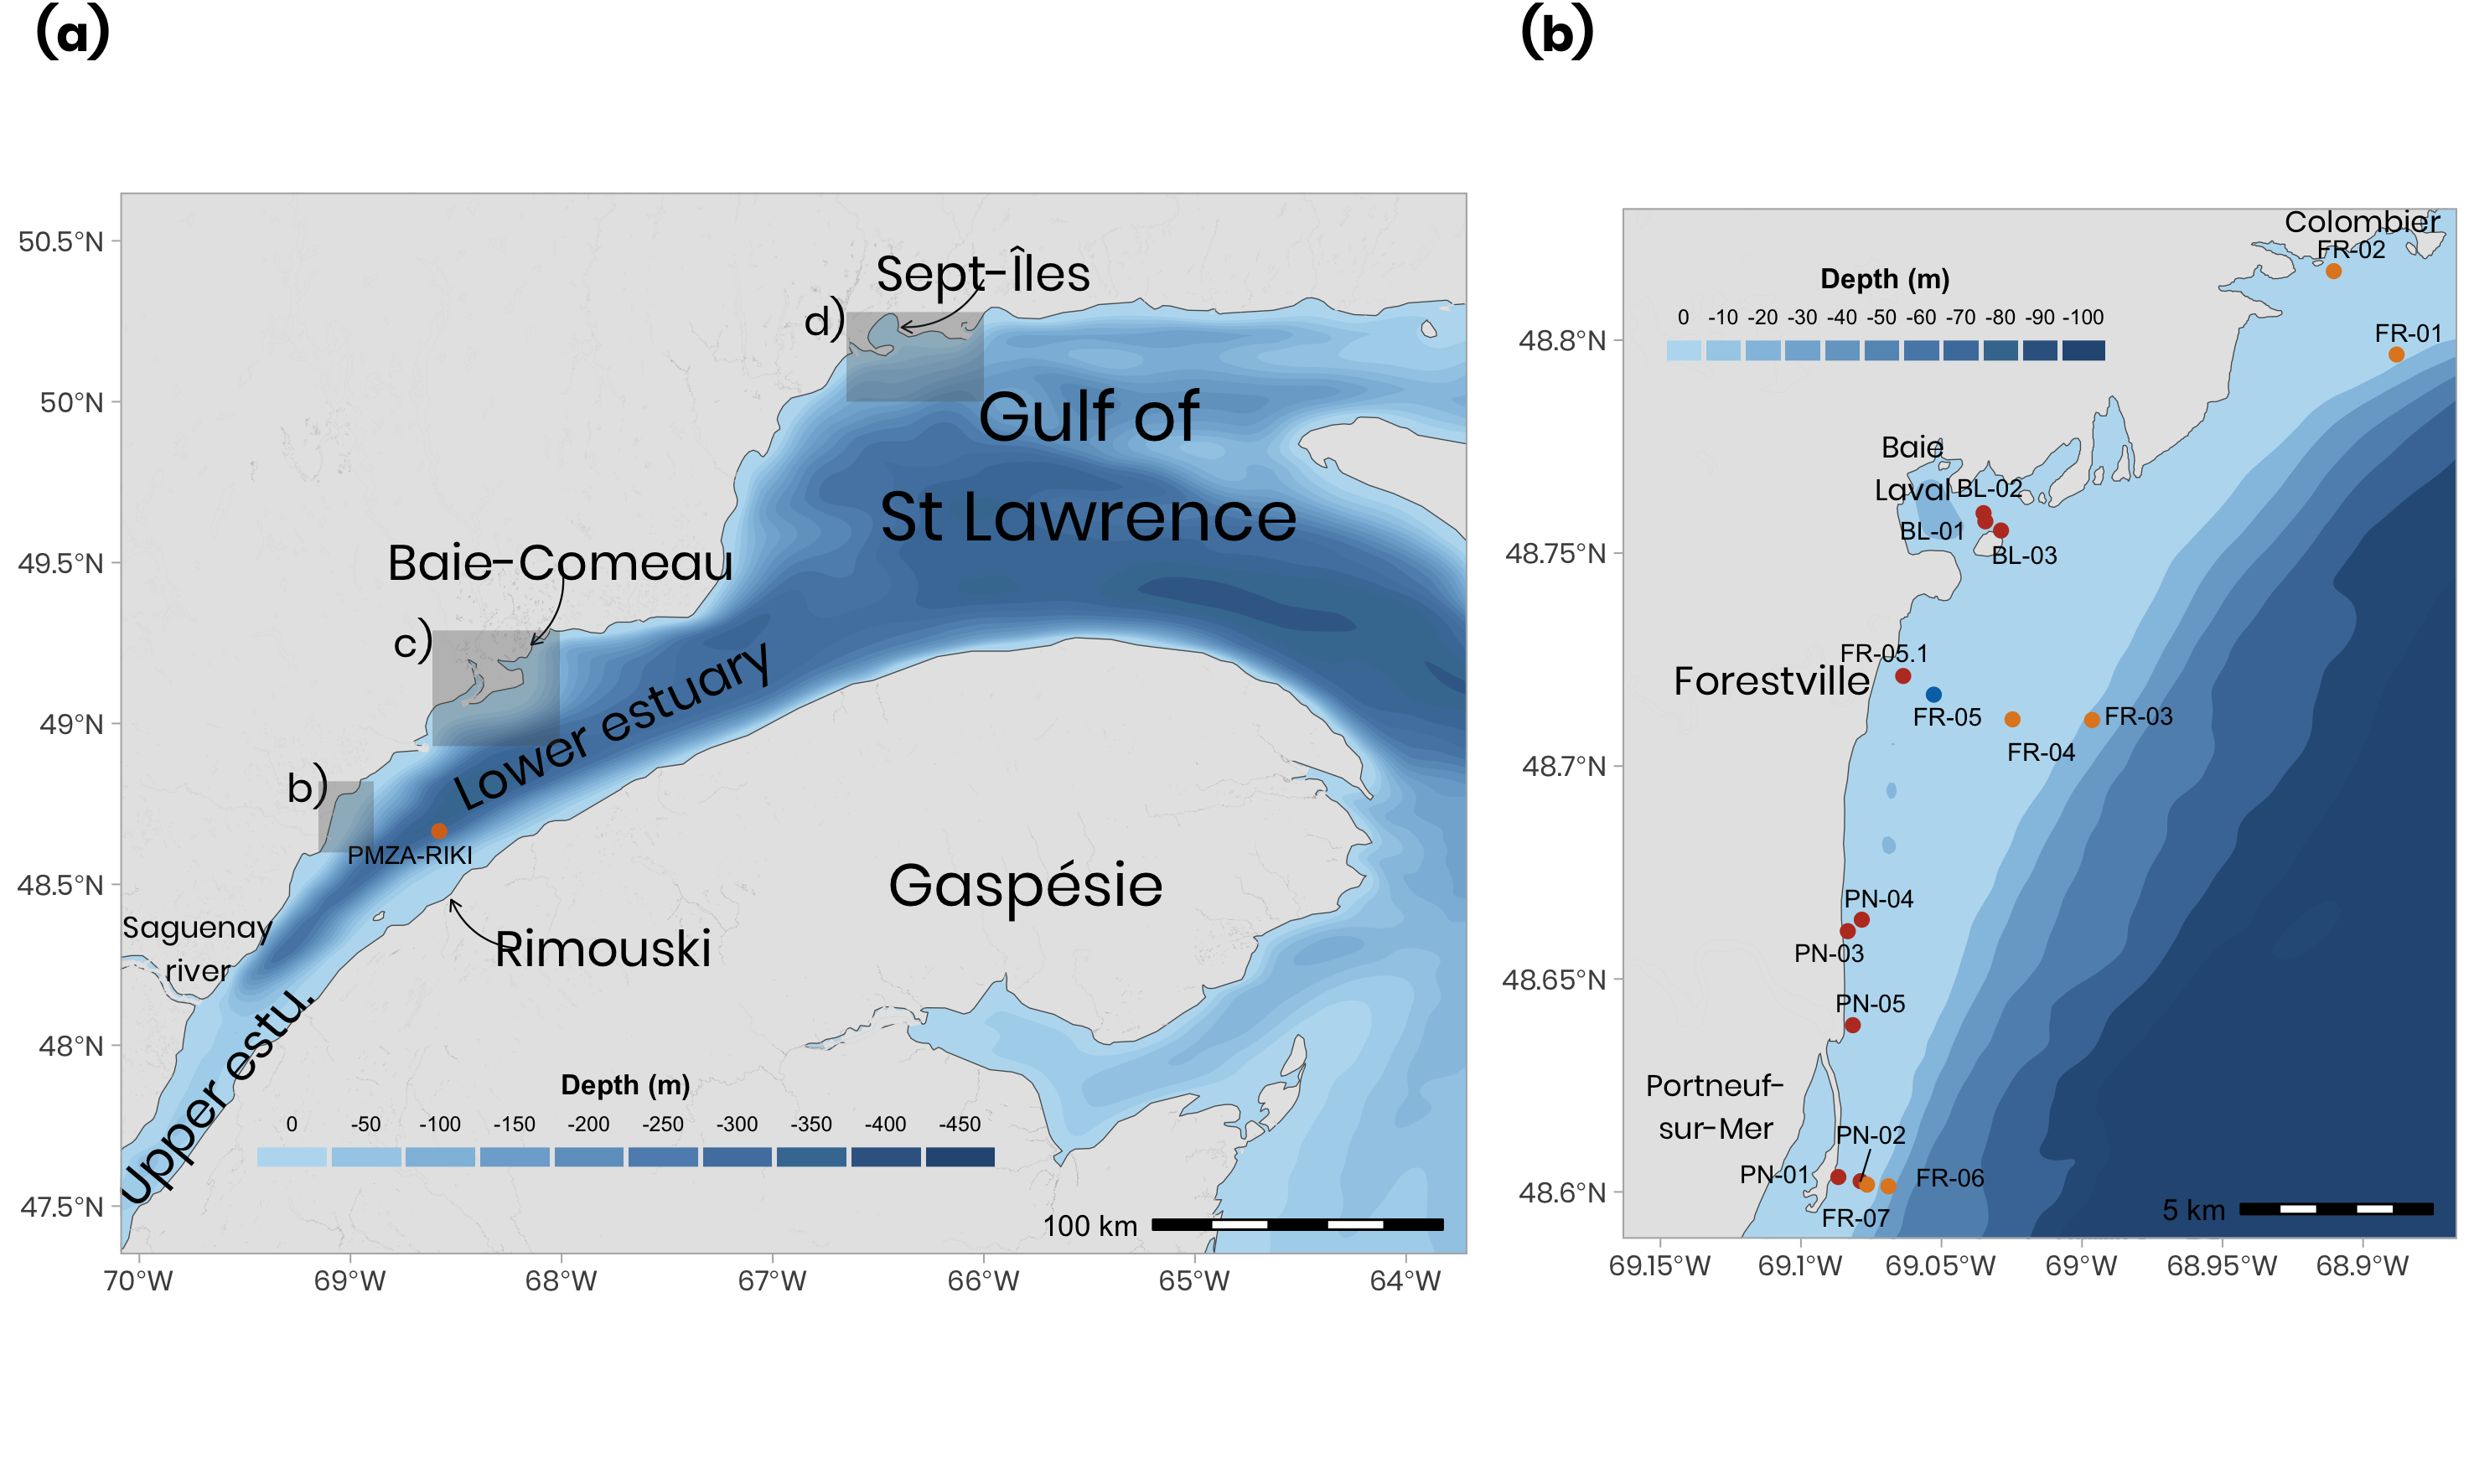
\includegraphics[width=12cm]{Figures/Fig1a-b.png}
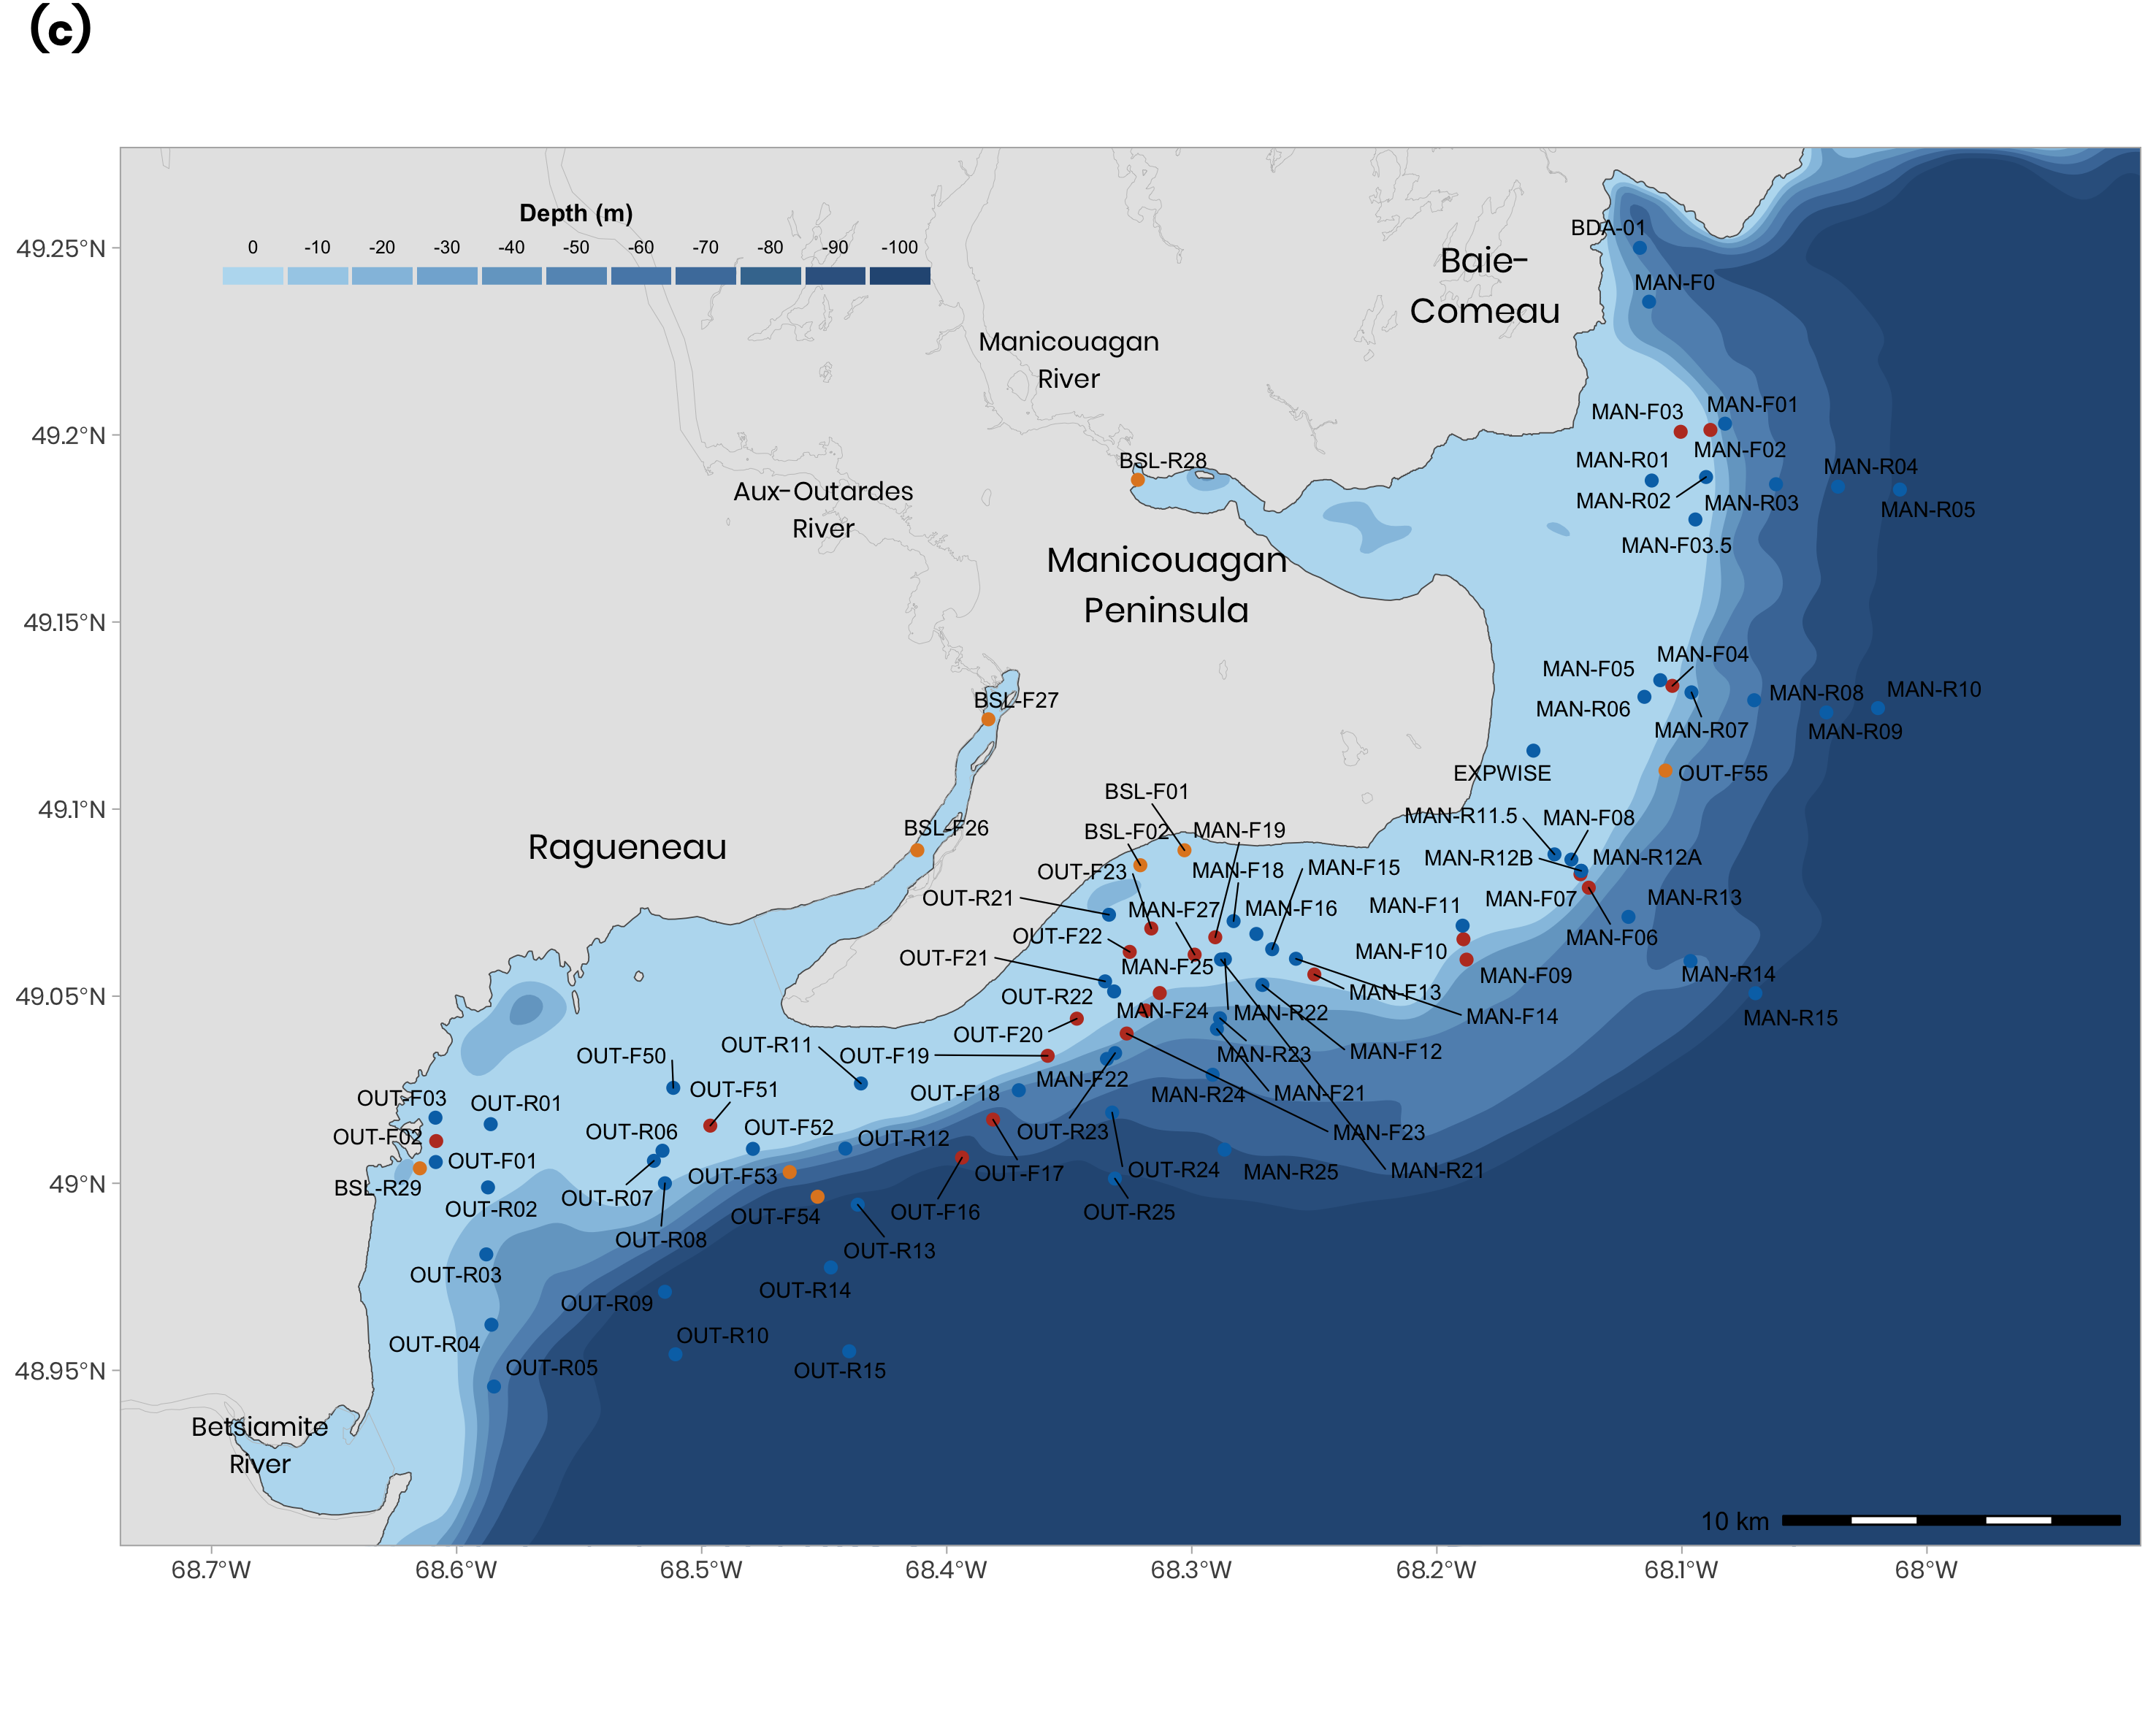
\includegraphics[width=12cm]{Figures/Fig1c.png}
\caption{Maps of stations where apparent optical properties (AOPs) have been determined. Insets in (a) are presented in (b) for the Forestville-Portneuf-sur-mer area visited on September 11 2017, (c) the Manicouagan Peninsula visited in August 2019, and (d) the Sept-Iles area visited on 11 occasions between August 2016 and June 2019. The color points indicate how the remote sensing reflectance was measured: in-water only (orange), above-water only (red) or both methods (blue).}
\label{fig:maps}
\end{figure}
\setcounter{figure}{0}
\begin{figure}[!ht]
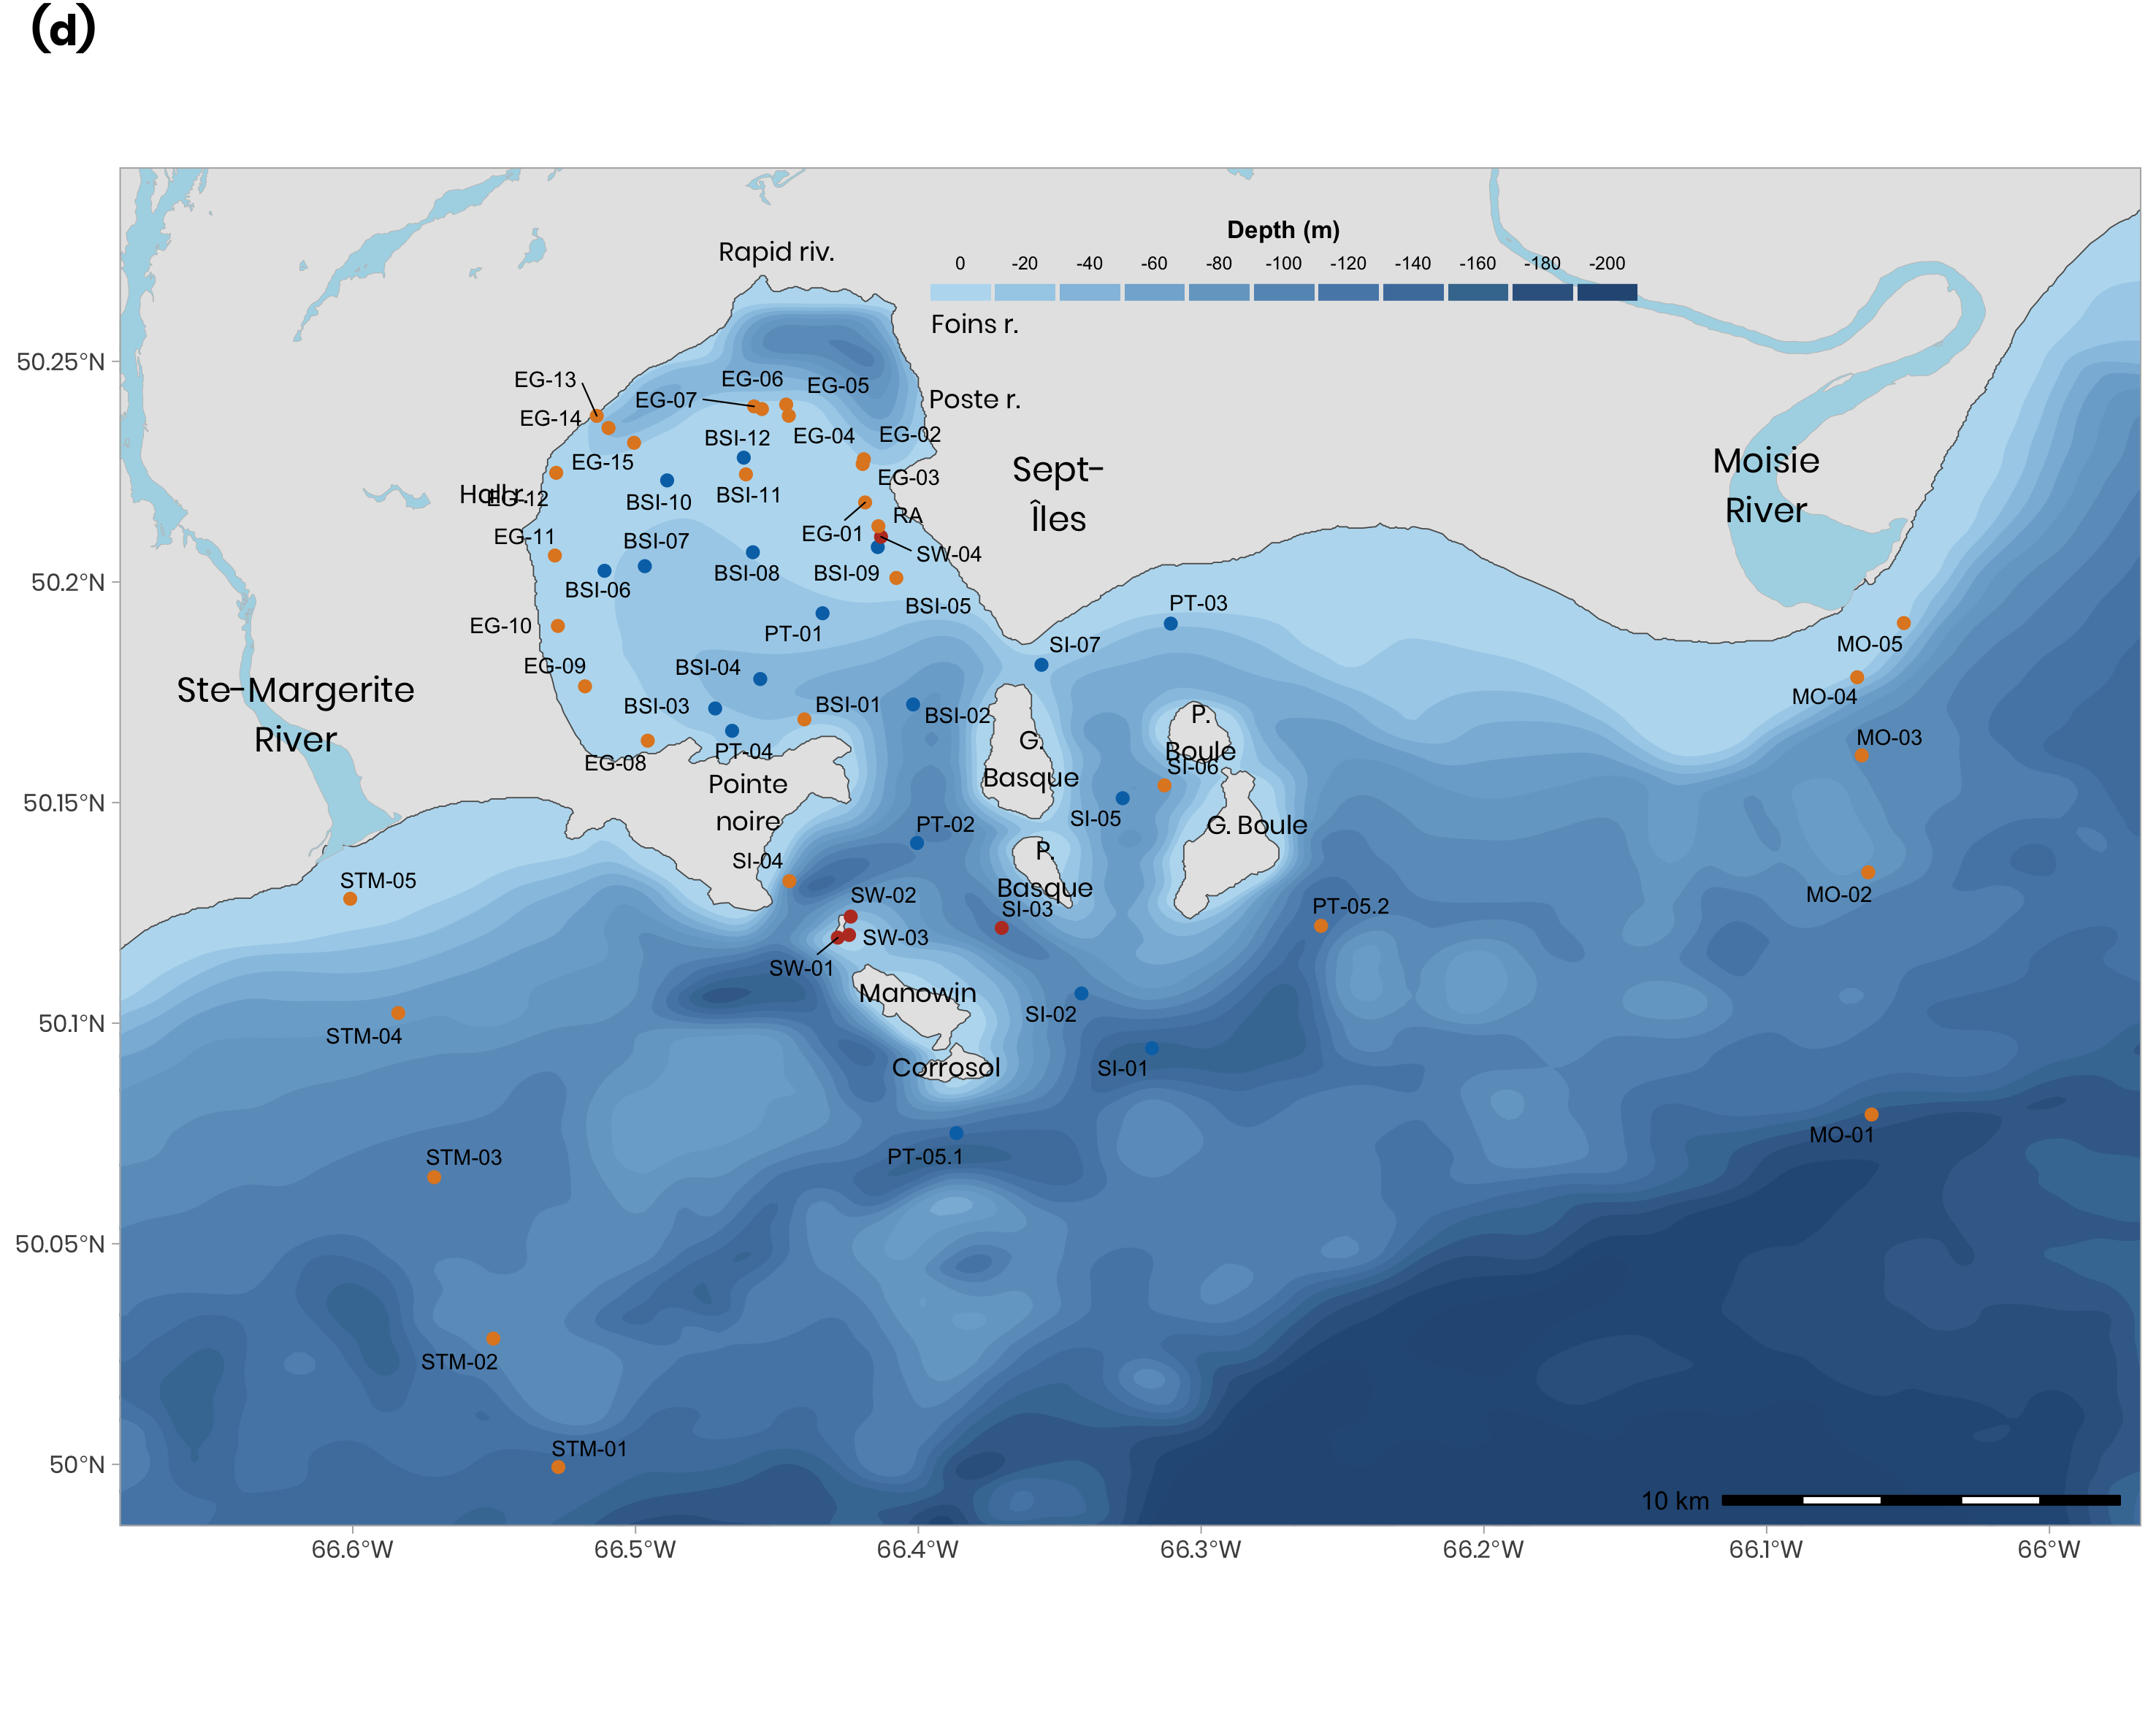
\includegraphics[width=12cm]{Figures/Fig1d.png}
\caption{Continue}
\end{figure}

\subsection{Atlantic Zone Monitoring Program : St Lawrence estuary autonomous buoy}
\label{sec:AZMP}
The Atlantic Zone Monitoring Program (AZMP) of DFO (or Programme de Monitorage de la Zone Atlantique [PMZA]) includes a network of autonomous oceanographic buoys across the coastal waters of the Maritime provinces of Canada. The station named PMZA-RIKI (Figure~\ref{fig:maps}a) in the SLE, just in front of Rimouski, has been visited on a regular basis (once a week in summer) since 1991. It was the first station to be instrumented with an autonomous buoy in 2002, including multispectral sensors dedicated to satellite validation of radiometric products. In 2015, we assessed the quality of the radiometric measurements available at the PMZA-RIKI buoy station in order to use these data for the validation of operational ocean color radiometric products \citep{Belanger2017}. The station was visited on 18 occasions between June 3$^{rd}$ and November 5$^{th}$ 2015, two times in 2016 (August 11 and 19), and once in 2017 (May 17) onboard DFO small (i.e. 30-foot length) craft boats (Table \ref{table:datasummary}).  On each occasion, 3 to 5 light profiles were carried with a Compact-Optical Profiling System (C-OPS) next to the buoy to determine the AOPs. An optical package, which included a CTD (conductivity-temperature-depth; SBE19 from Seabird scientific) and optical instruments (Hydroscat-6p, a-sphere), was deployed for the determination of inherent optical properties (IOPs). After the instrument package deployment, surface waters were sampled using a clean 20-L carboy kept in an iced cooler until it was processed in the Université du Québec à Rimouski (UQAR) laboratories the same day. Several physicochemical, biological and optical variables were determined from the discrete water samples. This data set was partially presented in \citet{Belanger2017} where more details about the sampling strategy can be found.\\ 

Unlike most coastal stations located along the northern shore of St Lawrence presented below, the estuarine waters found at the PMZA-RIKI station is under the influence of the St Lawrence river and the coastal up-welling taking place a the head of the Laurentian Channel near Tadoussac at the mouth of the Saguenay Fjord (Figure~\ref{fig:maps}a). This station increases the range of optical conditions encountered in the nearshore data set presented below.   
 
 \afterpage{%
    \clearpage% Flush earlier floats (otherwise order might not be correct)
    \thispagestyle{empty}% empty page style (?)
    \begin{landscape}% Landscape page
        \centering % Center table
        \begin{table}[t]
            \caption{Summary of field campaigns/projects including the number of stations, measurements and water samples.}
            \centering
            \begin{tabular}{ p{2cm}|p{2cm}|c|p{1.cm}|c|p{1.cm}p{1.cm}p{1.cm}p{1.cm}|p{1.cm}p{1.cm}p{1.cm}p{1.2cm}  }
            \tophline
            Area & Research project & Year & N. of campaigns & Dates &
            \multicolumn{4}{c|}{Number of stations} &
            \multicolumn{4}{c}{Number of measurements}\\
            \middlehline
             & & & & & Sea & River & Intertidal & Infra. & In-water radiom. & Above-water radiom. & IOPs & Surface (Sub-surface) sampling \\
            \middlehline
            SLE (PMZA-RIKI station) & Atlantic Zone Monitoring Program (AZMP) & 2015 & 18 & Jun-Nov & 1 & NA & NA & NA & 18 & 0 & 12 & 19 \\
            & & 2016 & 2 & Aug & 1 & NA & NA & NA & 3 & 0 & 0 & 0 \\
            & & 2017 & 1 & May & 1 & NA & NA & NA & 1 & 0 & 1 & 0 \\
            \middlehline
            Baie of Sept-Iles (BSI) & CHONe-2 & 2016 & 1 & Aug  & 9 & 3 & NA & NA & 9 & 0 & 0 & 12\\
            & & 2017 & 9 & Apr-Oct & 26 & 5 & NA & NA & 63 & 0 & 54 & 101(9)\\
             & & 2019 & 1 & Jun & 40 & 5 & NA & NA & 32 & 0 & 23 & 42 \\
             & $\mu$CASI & 2017 & 1 & Sep & 26 & 0 & NA & NA & 7 & 10 & 7 & 6\\
            \middlehline
            Forestville-Portneuf-sur-mer & $\mu$CASI & 2017 & 1 & Sep & 16 & NA & NA & NA & 7 & 10 & 7 & 6\\
            \middlehline
            Manicouagan & WISE-Man & 2019 & 1 & Aug & 89 & 3 & 195 & 7 & 59 & 84 & 63 & 70(15)\\
            \bottomhline
            \end{tabular}
            \label{table:datasummary}
        \end{table}
        %\captionof{table}{Table caption}% Add 'table' caption
    \end{landscape}
    \clearpage% Flush page
}
 
\subsection{Canadian Healthy Ocean Network (CHONe-2): Baie of Sept-Îles (BSI) project}
Within the scope of CHONe-2 funded by the Natural Sciences and Engineering Research Council of Canada (NSERC), 11 field campaigns were conducted in the Bay of Sept-Iles area from August 2016 to June 2019 (Figure~\ref{fig:maps}d, Table \ref{table:datasummary}).  The general objective of the CHONe-2 project in the BSI was to assess the potential stress of industrial and port activities on the coastal ecosystem, including vegetated habitats (eelgrass meadows and macroalgae), and benthic and pelagic ecosystems \citep{Ferrario2022}. A specific goal was to establish a bio-optical data baseline to promote and develop optical remote sensing tools for monitoring purposes at the bay scale \citep[for details see][]{Araujo2022a, Araujo2022b}.\\

Between 12 and 45 stations were visited on a given year in the BSI area (Table \ref{table:datasummary}). Bio-optical data was gathered both inside and outside the BSI, as well as on five rivers: four inside (Hall, au Foin, des Rapides and du Poste) and one outside the bay (Moisie river) (Figure~\ref{fig:maps}d).  The sampling at sea was made on a fisherman boat based at the Sept-Iles port. Typical measurements at sea involved radiometric vertical profiles for AOPs (C-OPS) and IOPs profiles (same optical package as described in section\ref{sec:AZMP}) and water sampling for laboratory analysis. The water sampling at sea was taken mostly at the surface using a bucket, but in 2017 some subsurface was sampled using a niskin bottle. Rivers were accessed from the main roads and measurements were made with a multiparameter probe and surface water collected with buckets.\\

AOPs and IOPs, as well as parameters measured from water samples, varied from one station to another mainly because of instrument availability.   Overall, a total of 56 unique sea stations and 5 river stations were repeatedly visited from 2016 to 2019. As a result, 104 measurements were made at sea for AOPs and 164 water samples (155 from surface, 9 from subsurface) were analysed for physico-chemical and bio-optical parameters.\\

\subsection{Hyperspectral remote sensing of optically shallow and coastal waters: $\mu$CASI and WISE-Man projects}
In September 2017, with the collaboration of DFO and the Canadian Hydrographic Service (CHS), fieldwork was carried along the northern shore of the EGSL in support of airborne hyperspectral imagery acquisition. The main objective of these acquisitions was to map the nearshore coastal habitats (e.g. eelgrass meadows, macroalgae, saltmarsh) and derived bathymetry of the nearshore zone. The $\mu$CASI sensor was flown on September 11 2017 by the IIC company in the Forestville area (Figure~\ref{fig:maps}b) and on September 14 2017 in the BSI area (Figure~\ref{fig:maps}d). The stations in the BSI were sampled as part of the CHONe-2 field campaigns described above (n = 26 stations, Table \ref{table:datasummary}). In Forestville area,  a total of 16 stations were visited (Table \ref{table:datasummary}). Above-water radiometry was measured using an ASD (Analytical Spectral Device) spectroradiometer with a small zodiac. In-water radiometry was measured with the C-OPS and surface water was sampled for basic bio-optical and biogeochemical variables (i.e., SPM, chlorophyll-a, CDOM and particulate absorption coefficients). Details on the number of stations and measurement types are given in Table~\ref{table:datasummary}.\\
 
In August 2019, an intensive field campaign was organized within the framework of the WaterSat Imaging Spectrometer Experiment (the \textit{WISE-Man project}; \textit{Man} stands for \textbf{Man}icouagan) in collaboration with several federal departments (Fisheries and Oceans Canada, National Research Council, Defence Research and Development Canada) and universities (UQAC, Laval, Boston). %a project supported by the Flights and Fieldwork for the Advancement of Science and Technology (FAST) program of the Canadian Space Agency (CSA), the Réseau Québec Maritime (RQM) and the DFO Ocean Protection Plan baseline program.  
The project main's objective was to demonstrate the potential of hyperspectral imagery for mapping bathymetry, water column quality (or IOPs), and retrieve bottom properties in order to respond to the pressing needs of science (e.g. ecology, geomorphology, coastal risk), resource management and defense operations.  In particular, the goal was to assess the performance of the WISE camera, a prototype sensor developed by ITRES inc. (Calgary, Canada) within the WaterSat initiative of the Canadian Space Agency (CSA). The campaign was conducted in the Manicouagan Peninsula, near Baie-Comeau, along the northern shore of the St Lawrence Estuary (Figure~\ref{fig:maps}c). A total of 92 stations were visited between August 17 and 25 2019 for bio-optical characterization using four small boats (Table \ref{table:datasummary}). The WISE sensor was flown on August 18 and 20th, 2019. Figure~\ref{fig:maps}c distinguishes the stations visited during the airborne surveys (e.g., MAN-Fx, OUT-Fx) from those visited the other days (e.g. MAN-Rx, OUT-Rx). At 64 out of 92 stations, CTD and \textit{in situ} IOPs were measured using two different instrument packages, and surface water was sampled using either a 5 L Niskin or a 4.2 L Wildco Beta horizontal sampler, both fired at about 0.5 m (surface; N = 64) or 4 to 5 m depth (sub-surface; N = 15, Table \ref{table:datasummary}). Two stations were sampled twice for water (EXPWISE and BDA-01) and six additional stations were sampled directly at the surface using a 20-L carboy from a small zodiac in rivers or very shallow waters, for a total number of 85 discrete water samples  (Table \ref{table:datasummary}). Finally, sea bottom habitats from intertidal and infra-littoral zones were characterized. The intertidal zone was characterized at low tide between July 27 and August 8 2019 at 195 stations (Figure~\ref{fig:intertidal}, Table \ref{table:datasummary}), while seven locations in the infra-littoral zone were sampled by a SCUBA diving team.  In addition to ecological, biological and physicochemical observations, hyperspectral reflectance measurements (emerged or submerged) were performed at most locations.\\  

\begin{figure}
    \centering
    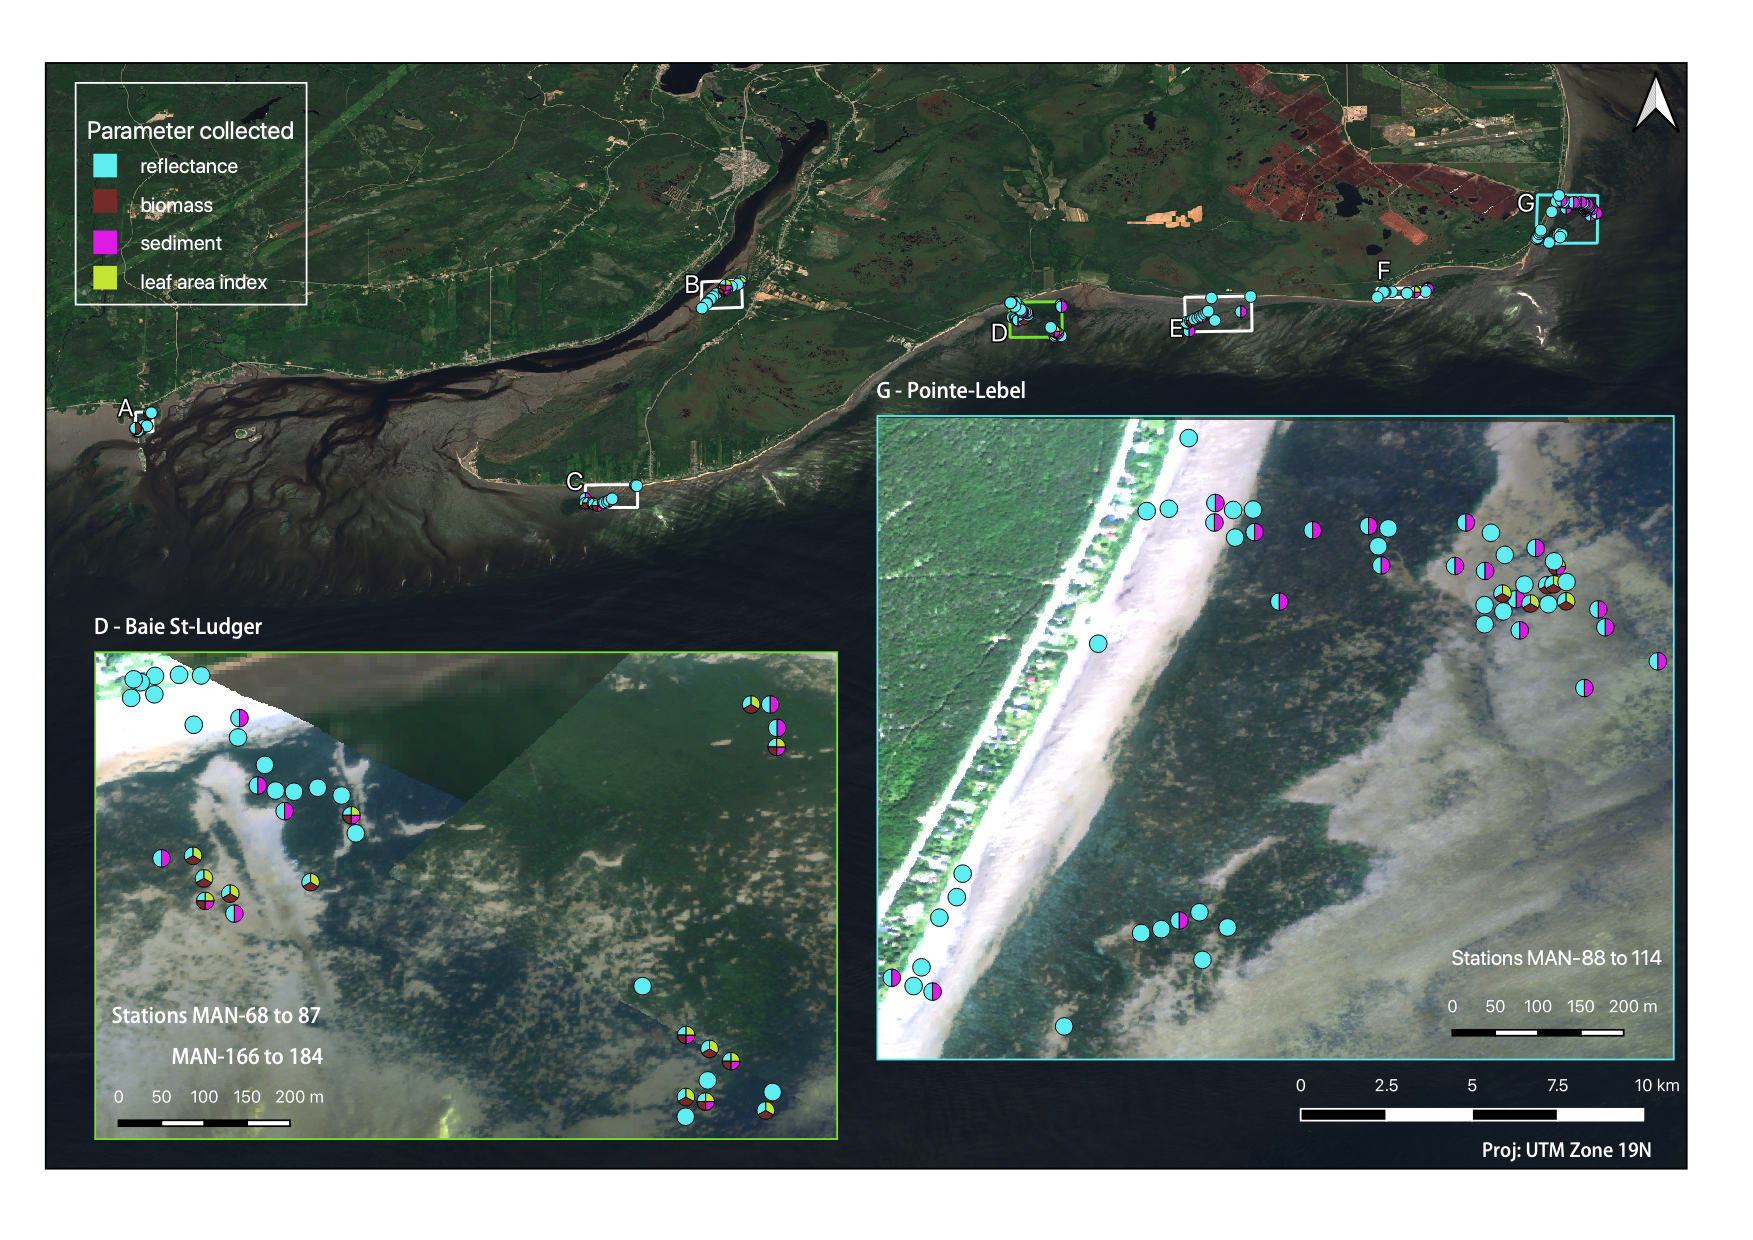
\includegraphics[width=15cm]{Figures/Fig2_intertidal_v3.png}
    \caption{Inter-tidal stations visited at low tide between July 27 and August 8, 2019 in the Manicouagan peninsula, showing the different parameters sampled. Insets are zoomed in for two sectors (D and G) out of seven (maps for sectors A,B,C,E and F are available in Appendix ~\ref{appendixfig}. }
    \label{fig:intertidal}
\end{figure}


\section{Material and methods}
This section provides a detailed description of the material and methods adopted for \textit{in situ} observations at each station (section~\ref{insitu}, including AOPs, IOPs and sun photometry), biogeochemical parameters on discrete water samples (section~\ref{labo}) and benthic habitats characterization (section~\ref{benthos}). Most material and methods are common to all projects presented above, but any project-related differences are pointed out when appropriate. 

\subsection{\textit{In situ} observations on stations} \label{insitu}
Typically, the following operations were performed at sea at a given station (note that the actual order may change depending on the time of the day or the sea state):
\begin{itemize}
  \item Three to five vertical profiles are done with the C-OPS for in-water AOPs determination.
  \item One vertical profile is made with an instrument package that includes at least a CTD and various active optical sensors for IOPs determination.
  \item When available, additional vertical profiles are made for multiparametric measurements (e.g., CTD, in vivo chlorophyll fluorescence, CDOM fluorescence, pH, oxygen, turbidity, etc).
  \item When available, above-water radiometry measurements using handheld spectroradiometer are performed to determine the hyperspectral remote sensing reflectance, $R_{rs}(\lambda)$. 
  \item Wind speed and direction is recorded for later processing. 
  \item When available and under clear sky, sun photometry is performed using a Microtops to determine the atmospheric aerosol optical depth ($\tau_a$) and water vapor content (WISE-Man only).
  \item Finally, surface water ($\sim$20-L), and on some occasions sub-surface water, is sampled using a bucket or an in-water sampler at 0.5 to 1 m depth. The water samples were kept in the dark in a cooler until processed in the laboratory, i.e., within 12 hours after sampling.
\end{itemize}

AOPs are those properties that are determined using radiometric measurements and that depend upon the ambient light field, the IOPs and the boundary conditions (sea state and bottom reflectance) \citep{Preisendorfer1961}.  Some of them, such as the diffuse attenuation coefficient of downwelling irradiance ($K_d$) can only be determined from in-water vertical radiometric profiles, while others, such as the remote sensing reflectance $R_{rs}$, can be determined using either in-water or above-water radiometric measurements.  Here we describe both approaches and give the main particularities of each instrument employed to determine the AOPs in our data set.\\  

\subsubsection{In-water radiometric profiles and AOPs determination}

\textbf{Compact-Optical Profiling System (C-OPS)}\\
The main instrument used to determine in-water AOPs, common to all projects, is the C-OPS (Biospherical Instruments)\citep{Hooker2013, Morrow2010}. All together, the data set contains 216 different stations totalizing $\sim$1000 C-OPS profiles. The C-OPS measures the light field in the water column with very high precision and accuracy at a frequency of 15 Hz. The C-OPS  measures the downwelling irradiance and the upwelling radiance in the water column at 19 wavebands ($\lambda$), i.e. $E_d(z,\lambda)$ and  $L_u(z,\lambda)$) where $z$ is depth. Simultaneous above-surface downward irradiance ($E_d(0+, \lambda)$) was measured with a radiometer attached on top of the boat making sure that no obstructions were in the field of view. In 2017, a CEREBUS frame was purchased by UQAR to deploy a third in-water sensor for upwelling irradiance, $E_u(z,\lambda)$. The wavebands for the UQAR's C-OPS are presented in Table~\ref{table:COPSwave} (note that the 305 nm channel was replaced by a 875 nm channel before the 2016 field season).  In 2019, a second C-OPS from Boston University (Dr Cedric Fichot) was used during the WISE-Man mission (35 stations), which has 16 common channels with the current UQAR's instrument setting (Table~\ref{table:COPSwave}). Both C-OPS were calibrated by the manufacturer on a yearly basis. 

\begin{table}[t]
\caption{Wavebands available on the two C-OPS systems.}
\centering
\begin{tabular}{ m{2.5cm}m{2.5cm}|m{2.5cm}  }
\tophline
\multicolumn{2}{c|}{UQAR (SN 13)} &
Boston University \\
\middlehline
2015 & 2016-2019 & 2019 \\
\middlehline
305  & NA  & 305 \\
320 & 320 & 320 \\
330 & 330 & NA \\
340 & 340 & 340 \\
380 & 380 & 380 \\
NA & NA & 395 \\
412 & 412 & 412 \\
443 & 443 & 443 \\
465 & 465 & 465 \\
490 & 490 & 490 \\
510 & 510 & 510 \\
532 & 532 & 532 \\
555 & 555 & NA \\
NA & NA & 560 \\
589 & 589 & 589 \\
625 & 625 & 625 \\
665 & 665 & 665 \\
683 & 683 & 683 \\
694 & 694 & 694 \\
710 & 710 & 710 \\
780 & 780 & 780 \\
NA & 875 & NA \\
\bottomhline
 \end{tabular}
 \label{table:COPSwave}
\end{table}

As mentioned above, three to $\sim$five C-OPS profiles were performed at each station. Most of the time, the boats were drifting during the measurements and the instrument was kept outside any disturbance or boat shadow. In very shallow waters (z $<$ 3 m) where tidal currents were strong, the boats were anchored to stay on station, allowing the profiler to drift away from the boat shadow. The C-OPS data were processed in R software with the \texttt{Cops} library first developed by Dr. B. Gentili at the Laboratoire d'Océanographie de Villefranche (LOV) and now maintained by Dr S Bélanger (the source code is available at \url{https://github.com/belasi01/Cops}). The data processing respects the NASA protocols \citep{Mueller2003}, but additional features have been developed to optimize the data processing in R. AOPs were derived from vertical profiles of downward irradiance ($E_d(z,\lambda)$), upward radiance ($L_u(z,\lambda)$), and when available, upward irradiance ($E_u(z,\lambda)$). Each profile was carefully inspected and records showing high instrument tilt were discarded, i.e. $> 5^{\circ}$ for in-water quantities and $> 10^{\circ}$ for $E_d(0+,\lambda)$. To get enough data points in the first-meter of water to obtain a precise extrapolation of the radiometric quantities at the sea-air interface ($z=0-$), we often have to relax the tilt limit threshold to 7 or 8$^{\circ}$ for the upwelling quantities (i.e., $E_u(z,\lambda)$ and $L_u(z,\lambda)$). In fact, high tilt is often encounter near the sea surface water, in particular in highly stratified and shallow waters due to higher currents and waves action. In addition, any radiometric quantities below the instrument detection limit were removed (i.e., noisy measurements). The latter varies between instruments and wavebands and were determined by the operator from deep C-OPS profiles. Typical values for the detection limit vary from \num{1e-4} to \num{7e-3} \si{\micro.W.cm^{-2}.nm^{-1}} for $E_d(z,\lambda)$ and $E_u(z,\lambda)$, respectively, and for \num{1e-5} to \num{2e-4} \si{\micro.W.cm^{-2}.nm^{-1}.sr^{-1}} for $L_u(z,\lambda)$. The detection limit is lowest in the visible bands and highest in the UV domain. In CDOM-rich waters, such as those characterizing the nearshore waters of the EGSL, the detection limit was often reached in the top 5 to 10 meters in the UV channels.\\ 

In-water radiometric quantities were normalized with respect to simultaneous measurements of the global solar irradiance in the air, $E_d(0+,\lambda,t)$, with $t$ explicitly expressing the time dependence, according to

\begin{equation}
\Xi(z,\lambda,t_0) = \Xi((z,\lambda,t))\frac{E_d(0+,\lambda,t_0)}{E_d(0+,\lambda,t)}
\label{eq:xi}
\end{equation}

where $\Xi$ identifies the radiometric quantity (i.e., $E_d(z,\lambda)$, $E_u(z,\lambda)$ or $L_u(z,\lambda)$) that is normalized to account for incident irradiance fluctuations during the vertical profiles induced by the atmospheric conditions. After the normalization and filtering of $\Xi$, an extrapolation of the quantities of interest just below the sea surface ($z=0-$) is performed using two approaches: 

\begin{enumerate}
    \item $\Xi(z,\lambda,t_0)$ profiles are fitted using a linear regression applied to log-transformed radiometric quantity versus depth. The thickness of the surface layer ($\Delta z_{surf}$) considered for the extrapolation varied as a function of wavebands and the quality of the data fitting. It varied between 0.3 and 2.5~m (3.0 for $E_d(z,\lambda)$) below the very first valid C-OPS measurements in the water column (typically around 0.35 to 0.5~m depth for the upward quantities). For example, if $L_u(z,\lambda)$) measurements begin at 0.4 m depth, the minimum layer considered will extend from 0.4 to 0.7~m for $\Delta z_{surf}$ of 0.3~m, or from 0.4 to 2.9~m for $\Delta z_{surf}$ of 2.5~m. A linear model is fitted to the log-transformed $\Xi(z,\lambda,t_0)$ vs depth ($z$) to all layers from the minimum and the maximum thickness considered, starting with a minimum number of ten valid measurements and adding one observation at a time. The goodness of the fit is evaluated using the coefficient of determination ($r^2$) to all layers. In addition, we apply a Kolmogorov-Smirnov test to make sure the depth distribution within each layer is not bimodal and the free-fall is relatively constant, which can produce a high value of $r^2$ but poor fitting. The Kolmogorov-Smirnov test compares the actual $z$ distribution to an expected $z$ distribution, in which $z$ is evenly spaced from the minimum and maximum depth the layer considered. If the p.value $>$ 0.1, the $z$ distribution is considered not evenly spaced and the fit is not retrained% (even if it presents the highest $r^2$). 
    Otherwise, the layer presenting the highest $r^2$ is retrained for the linear extrapolation of $\Xi(z,\lambda,t_0)$. Finally, we imposed arbitrarily a lower limit for the $r^2$ of 0.5 to 0.6 for $E_u(z,\lambda)$ and $L_u(z,\lambda)$) and 0.5 for $E_d(z,\lambda)$. These thresholds can be adjusted by the operators in presence of noisy data due to wave focusing effect, which may result in very low $r^2$ and a failure of the linear extrapolation. In general, the thickness of the layers considered are thinner in the UV and near-infrared spectral domains. In summary, the linear extrapolation method is similar to that adopted by \citet{Antoine2013a} and was improved relative to that described in \citet{Belanger2017}. 
    \item A non-linear fitting method was also implemented in the \texttt{Cops} R package, known as LOESS (local polynomial regression fitting), which is a non-parametric method usually employed to smooth time-series (but here applied to light profile). LOESS computes polynomials on the data for a given moving window size (typically 3 to 5 meters depending on wavebands and vertical structure of the water column) along the profile. The LOESS fitting is particularly efficient for smoothing $\Xi$ profiles showing actual non-linear features introduced by either non-homogenous vertical profile (i.e., optically-stratified), the presence of bottom in optically shallow waters or the effect of inelastic scattering processes (e.g., sun-induced fluorescence in subsurface chlorophyll-a maximum layers).  LOESS fitting method could also be used to extrapolate $\Xi$ to $z=0-$. It is often preferable in optically shallow water where upwelling light is highly non-linear in the log-transformed domain (see below for example).  
\end{enumerate}

Next, $L_u(0-,\lambda)$ and $E_u(0-,\lambda)$ were corrected for instrument self-shadow following the procedure proposed by \citet{Gordon1992b} and \citet{Zibordi1995}, which requires the total absorption coefficients, $a_t$, at each C-OPS channels and the fraction of diffuse versus direct component of solar irradiance, $f_{diff}$. For most station, \textit{in situ} non-water absorption profiles were used. Otherwise, discrete measurements of CDOM ($a_g$) and particulate absorption ($a_p$) coefficients were used. In the rare case where \textit{in situ} and discrete absorption measurements were not available, total absorption was estimated from diffuse downwelling attenuation coefficient ($K_d$) and the sub-surface irradiance reflectance ($R$) computed for the surface layer using the analytical model described in \citet{Morel2001} (their eq. 8'). To obtain the fraction of diffuse versus direct component of solar irradiance, we used the data from the shadow band of the BioShade instrument attached to the reference sensor, as detailed in \citet{Belanger2017}. 
Briefly, the BioShade is a motor that moves a black aluminum band (shadowband) 1.5 mm thick and  2.5 cm wide back and forth above the reference sensor \citet{Morrow2010}. 
Under clear sky conditions, when the shadowband completely blocks direct sun at time $t_{shadow}$, the radiometer measures the diffuse skylight (minus a part of the sky that is also blocked by the shadowband), $E_d^{diff}(0+,\lambda,t_{shadow})$. When the shadowband is horizontal, the sensor measures the global solar irradiance, $E_d(0+,\lambda,t)$. So to assess the global solar irradiance at the time $t_{shadow}$, we interpolate $E_d(0+,\lambda,t)$ just before and after the shadowband started to shade the sensor. This allows to approximate the fraction of diffuse skylight to the total downwelling irradiance as : 

\begin{equation}
 \label{eq:diffuseEd}
f_{diff} = \frac{E_d^{diff}(0+,\lambda,t_{shadow})}{E_d(0+,\lambda,t_{shadow})}
\end{equation}
Because part of the sky is also blocked by the shadowband at $t_{shadow}$, $f_{diff}$ will be slightly underestimated. This underestimation have negligible impact on the calculations of the shading error \citep{Belanger2017}. In the absence of shadowband, \citet{Gregg1990} clear-sky irradiance model (hereafter refer to as GC90) was used to approximate $f_{diff}$. An iterative method was implemented starting with very clear atmosphere (through the $\mathrm{visibility})$ parameter) to simulate total downward irradiance at 490 nm ($E_d^{GC90}(490, \mathrm{visibility})$)  The $\mathrm{visibility})$ is reduced until measured $E_d(0+,490)$ == $E_d^{GC90}(490, \mathrm{visibility})$. When the equality is reach, the modelled total and diffuse components from GC90 are used to estimate $f_{diff}$. \\ 

Water-leaving radiance, $L_w(\lambda)$, was calculated from the extrapolated radiance just below the sea surface corrected for instrument shadow as:
 \begin{equation}
 \label{eq:L_w}
L_w(\lambda) = 0.54\,L_u(0-,\lambda)
\end{equation}
where the factor 0.54 accounts for the partial reflection and transmission of the upwelled radiance through the sea surface \citep{Mueller2003}. 
The remote sensing reflectance, $R_{rs}(\lambda)$, was computed as:
 \begin{equation}
 \label{eq:Rrs}
R_{rs}(\lambda) = \frac{L_w(\lambda)}{E_d(0+,\lambda,t_0)} 
\end{equation}

For a given date, the AOPs derived from three to five profiles were averaged after eliminating spectra that showed large discrepancy relative to the mean spectrum (i.e., if the difference between mean and replicates was $>$10\% in terms of $R_{rs}$).\\  

The AOPs data set also includes spectral diffuse attenuation coefficient of downwelling irradiance, $K_d(\lambda)$, as computed for two surface layers. Here we defined an average attenuation coefficient from the surface (0-) to the depth $z$ where the downwelling irradiance is reduced to 10\% or 1\% of its surface value measured just below the sea surface (i.e., $E_d(0-)$):  

\begin{equation}
    \overline{K_d}(0- \leftrightarrow z, \lambda) = \frac{1}{z}\ln \left( \frac{E_d(z, \lambda)}{E_d(0-, \lambda)} \right)
    \label{eq:Kd}
\end{equation}

Therefore, $\overline{K_d^{1\%}}(\lambda)$ and $\overline{K_d^{10\%}}(\lambda)$ were computed using eq~\ref{eq:Kd} for the depth $z$ where $\frac{E_d(z,\lambda)}{E_d(0-, \lambda)}$ yield a values of 1\% and 10\%, respectively. The calculation is based on $E_d(0-, \lambda)$ obtained from measured $E_d(0+, \lambda)$ times 0.97 to account for the air-sea transmittance \citep{Mueller2003} and vertical profiles of normalized $E_d(z, \lambda)$ (eq.~\ref{eq:xi}) and smoothed using the LOESS fitting method. As a result, the depth of the actual layer consider for $\overline{K_d}(\lambda)$ is wavelength dependent since the depth of the 1\% or the 10\% light level is spectrally dependent. \\ 

In optically shallow waters, the bottom reflectance ($R_b$) was extracted from C-OPS profiles at wavebands where the radiometric signal was above the detection limit at the bottom of the water column. We developped our own method to extract $R_b$ from C-OPS profiles, which is briefly presented here.   Figure~\ref{fig:Rb} presents an example of a C-OPS profile performed at a station on the Manicouagan Peninsula over a sandy bottom. First, the depth of the water column is estimated using the pressure sensor of the C-OPS when it sits on the bottom. In this example, the instrument was free-falling from the surface to the bottom when the pressure remained constant with time at 5.2~m depth (Figure~\ref{fig:Rb}a). For this station the total water column depth was 5.45~m after adding the distance between the pressure sensor and the base of the instrument (i.e., 0.25~m). All radiometric data in the first 15~cm above the bottom are contaminated by instrument shading and are systematically removed. Figures~\ref{fig:Rb}b and \ref{fig:Rb}c show the vertical profiles of $E_d(z, \lambda)$ and $L_u(z, \lambda)$, respectively, at three selected wavelengths in the visible (i.e., 443, 560 and 625 nm). While $E_d(z, \lambda)$ show a typical exponential decrease with depth at all wavelengths,  $L_u(z, \lambda)$ in the blue tend to level off at 3~m, and even increase slightly with depth in the green and in the red due to the bottom reflectance, which is higher than the water column reflectance itself. $R_b$ is estimated using the radiometric quantities measured 25~cm above the bottom (i.e., dashed line on Figures~\ref{fig:Rb}b and c):

\begin{equation}
    R_b(z = \mathrm{bottom-0.25~m}, \lambda) = \frac{\pi \times L_u(z = \mathrm{bottom-0.25~m}, \lambda)}{E_d(z = \mathrm{bottom-0.25~m}, \lambda)} = \frac{E_u(z = \mathrm{bottom-0.25~m}, \lambda)}{E_d(z = \mathrm{bottom-0.25~m}, \lambda)}
\end{equation}

\begin{figure}
    \centering
    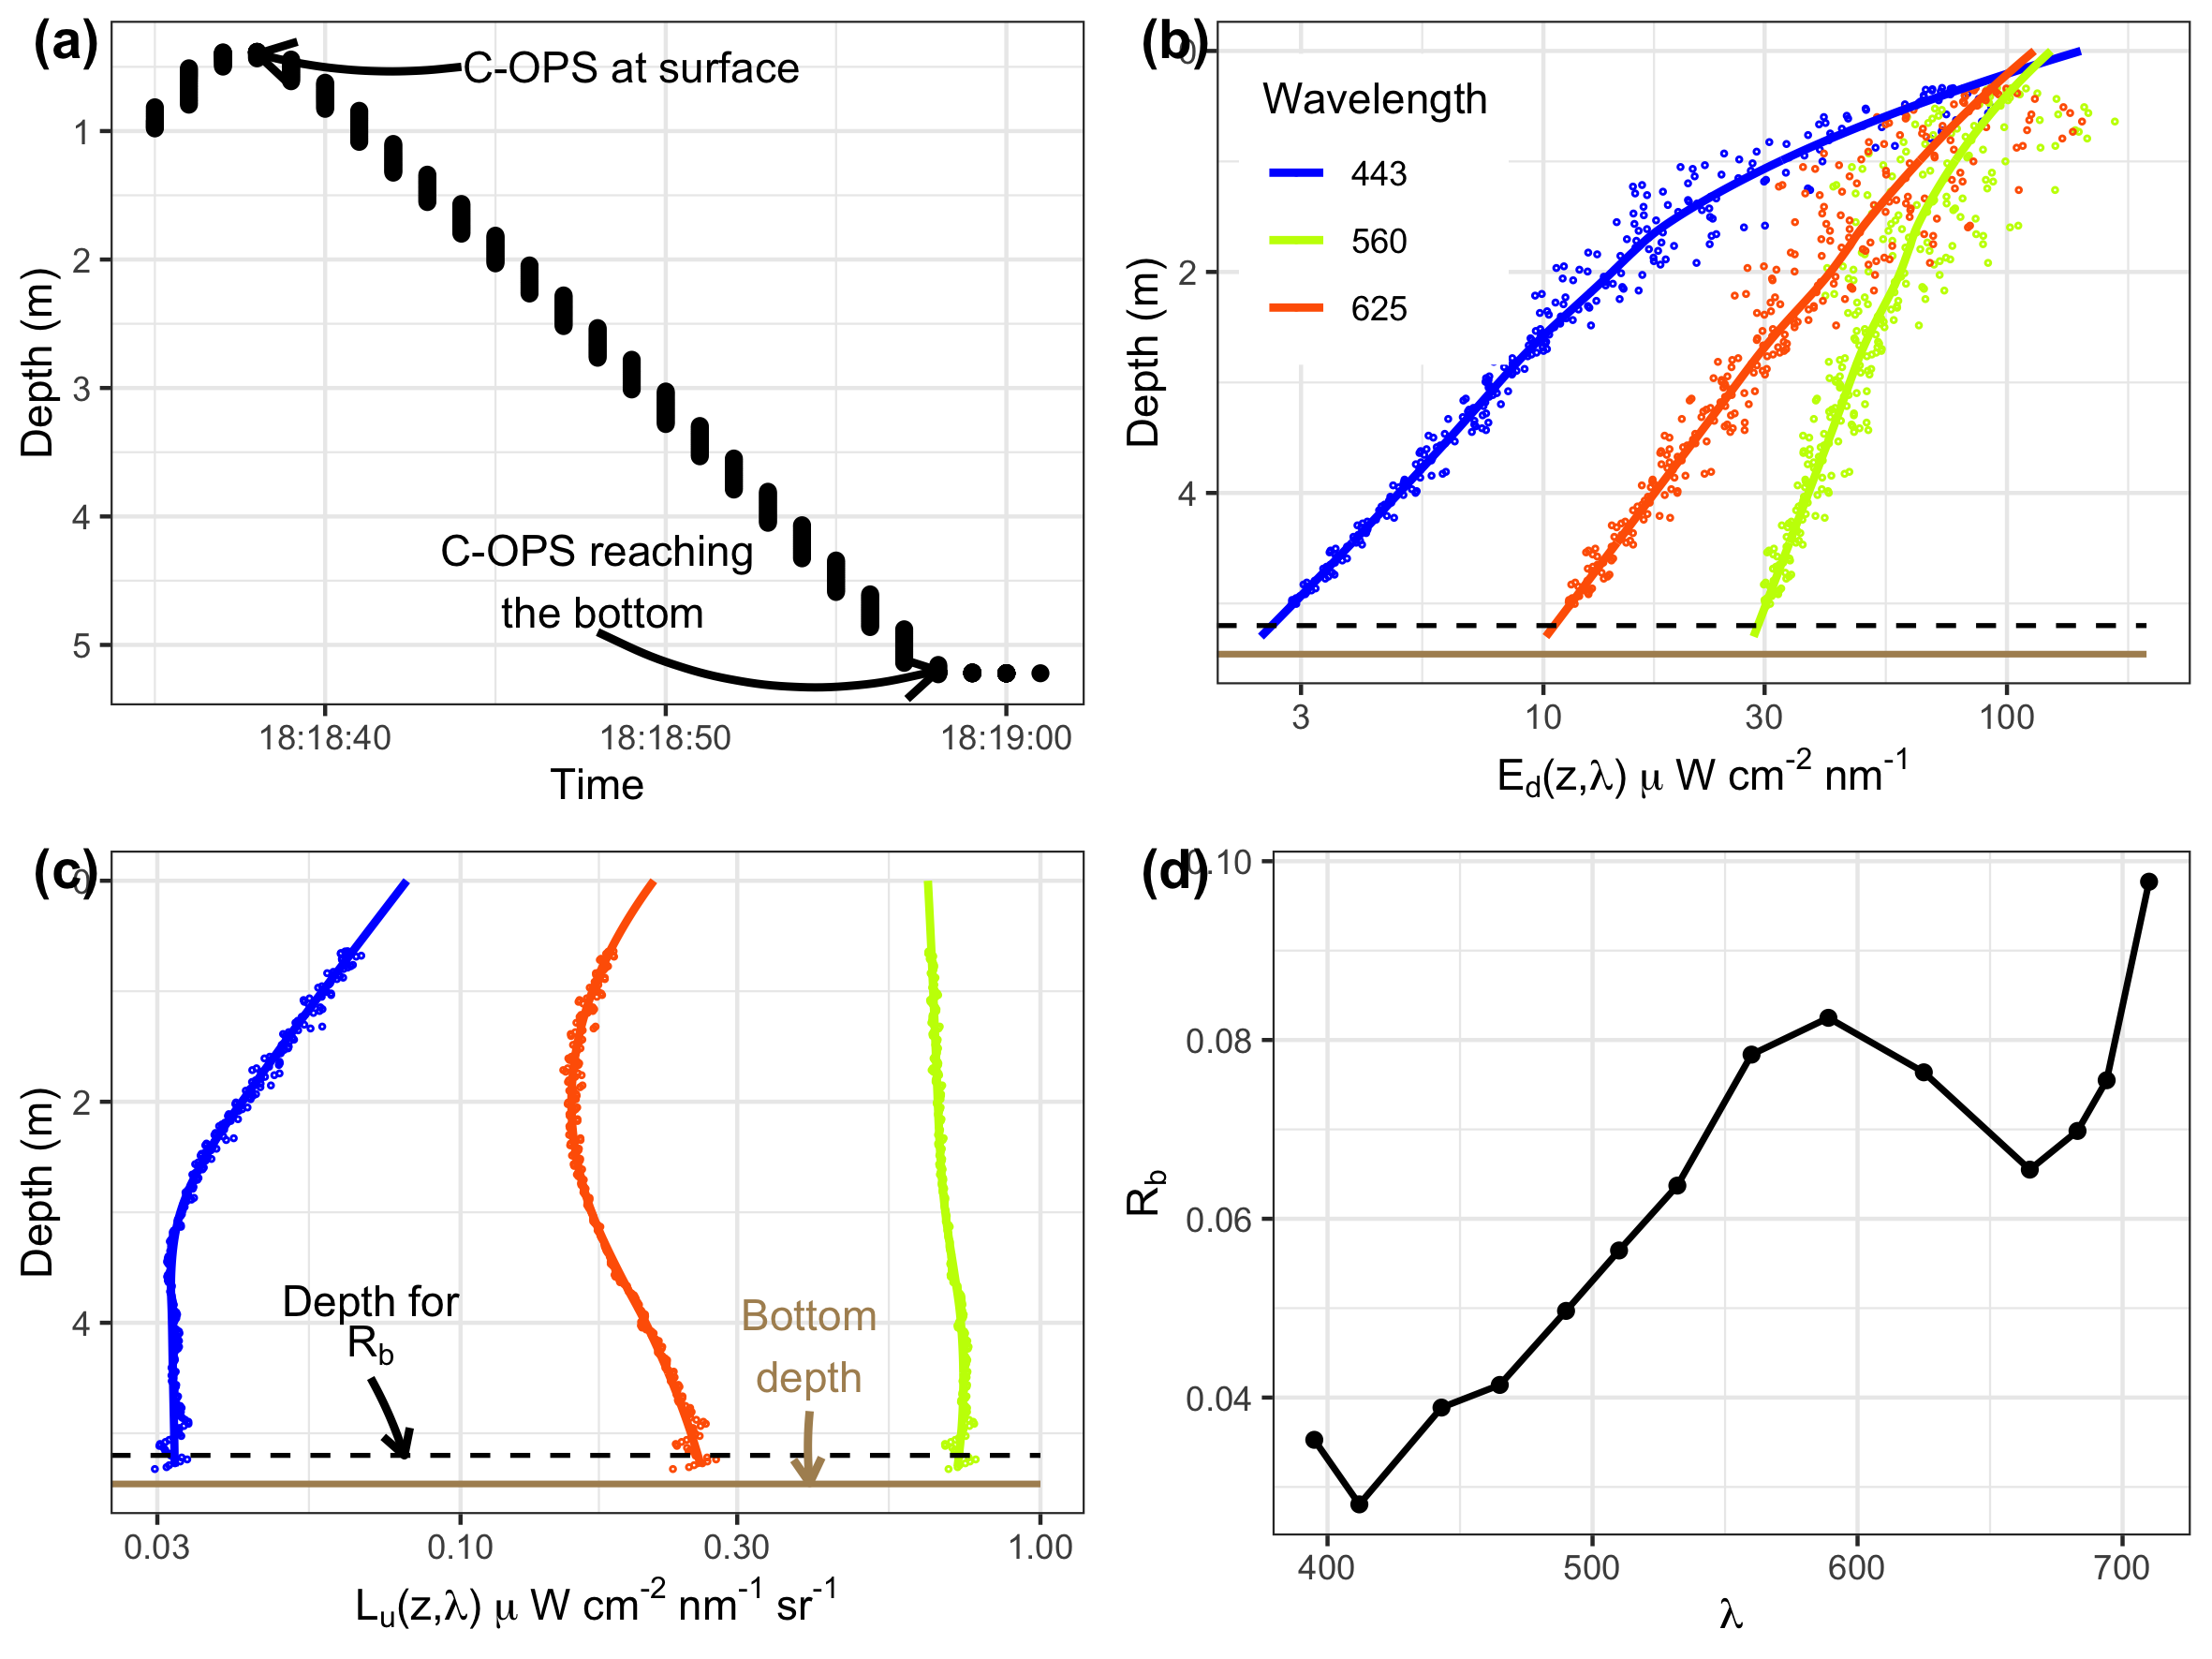
\includegraphics[width=18cm]{Figures/Fig_Rb.png}
    \caption{Example of an estimation of $R_b(\lambda)$  from C-OPS vertical profiles of $E_d(z,\lambda)$ and $L_u(z,\lambda)$, respectively.   }
    \label{fig:Rb}
\end{figure}
Figure~\ref{fig:Rb}d show the resulting $R_b(\lambda)$ of the MAN-F05 station (averaged from 3 C-OPS profiles). The spectral range $R_b(\lambda)$ in this example is restricted to 395 to 710 nm, and it was determined by the detection limit of each individual C-OPS channel. In other words, not enough light reach the bottom in the four UV channels (<380 nm) and in the near infrared channel at 780 nm.\\       

\textbf{HyperOCR}\\
In 2019, we adapted a Satlantic HyperSAS system to measure in-water hyperspectral $R_{rs}(\lambda)$ from small boats with the capacity to navigate in very shallow waters (see also \citet{Mabit2022}). The HOCR spectral range spans from 380 to 800~nm at 3~nm resolution. The radiometers were calibrated just before the deployment by the manufacturer. In-water upwelling radiance below the sea surface was measured using two hyperOCR radiometers (HOCR) held away from the boat with a pole and submerged at two different depths. The surface sensor was lowered at $\sim$5 to 15~cm depth, while the second sensor was $\sim$30~cm deeper (i.e., 40 to 55~cm depth). This set up, while avoiding the surface sky glint correction, allow the calculation of the attenuation coefficient of the up-welling radiance, $K_{L_u}(\lambda)$, which is needed to extrapolate $L_u(z,\lambda)$ to  $L_u(0-,\lambda)$. Note that $K_{L_u}(\lambda)$ is far from being constant with depth and can be positive in some part of the spectral and negative in other parts, as illustrate in Figure~\ref{fig:Rb}c. Simultaneously, incident $E_d(0^+)$ was measured above water using a radiometer attached to the side of boat above the structure to avoid shadow.\\  

HOCR data were processed using the open-source R-package HyperocR available on the GitHub platform (\url{https://github.com/belasi01/HyperOCR}). The processing includes the extrapolation of $L_u(z,\lambda)$  to the sea surface using estimated value of $K_{L_u}(\lambda)$ and its transmission across the air-water interface, which is used to estimate the $L_w(0^+, \lambda)$  and $R_{rs}(\lambda)$ (eqs.\ref{eq:L_w} and \ref{eq:Rrs}). Note that the instrument self-shadow correction was considered negligible for HOCR due to the small radius of the instrument (3~cm).  

\subsubsection{Above-water radiometry}
In support of airborne hyperspectral data acquisition, we performed above-water radiometric measurements in 2017 and 2019. Two spectroradiometers were used: an analytical spectral device FieldSpec HandHeld 2 (ASD) and a spectral evolution PSR-1100f (PSR). Both instruments had a spectral resolution of $\sim$3~nm covering a spectral range from 325/320 to 1075/1100 nm (ASD/PSR) and were fitted with a bare fiber optic with a 25\degree field of view (FOV). Calibrated spectralon panels were used as reference to compute the remote sensing reflectance following \citet{Mobley1999}: 

\begin{equation}
    \label{eq:Rrs_above}
    R_{rs}(\lambda) = (L_t(\lambda) - \rho_{sky}L_{sky}(\lambda)) / \left( \frac{\pi}{R_p(\lambda)}\times L_p(\lambda) \right) - \Delta
\end{equation}

where $L_t(\lambda)$ is the total upwelling radiance from the water as measured by the instrument; $\rho_{sky}$ is the skylight reflectance that depends upon the sun-viewing geometry, sea state (i.e., wind speed) and instrument FOV; $L_{sky}(\lambda)$ is the sky radiance coming from the direction of specularly reflected sky light; $L_p(\lambda)$ and $R_p(\lambda)$ are the up-welling radiance and reflectance of the spectralon panel, respectively; and $\Delta$ a residual . In general, a sequence of $L_t(\lambda)$, $L_{sky}(\lambda)$  and $L_t(\lambda)$ was made on a station and last for about 5 minutes. The instrument integration time and dark current subtraction were systematically apply for each radiance measurements. The sensor viewing zenith angle ($\theta_v$) of $\sim$40\degree and an azimuth difference between the solar and sensor ($\Delta\phi$) planes between 90 and 135\degree was chosen to minimize the sun glint contamination \citep{Mobley1999}. The windspeed and sun-view geometry was recorded systematically to perform the sky glint correction.   \\

Several methods were implemented and tested to estimate $\rho_{sky}$, including 
\begin{enumerate}
    \item Look-up-tables of $\rho_{sky}$ published by  \citet{Mobley1999,Mobley2015} taking as input the $\theta_v$, $\Delta\phi$, the sun zenith angle ($\theta_s$) and the wind speed (hereafter the LUT method);
    \item LUT method with a white correction using the residual values of $R_{rs}$ in the near infrared (890-900 nm) (assuming black waters in this spectral range); 
    \item LUT method with white correction assuming the similarity spectrum in NIR of \citet{Ruddick2006} using two NIR bands at 720 and 780 nm respectively (ideal for moderately turbid waters); 
    \item LUT method with white correction assuming the similarity spectrum in NIR of \citet{Ruddick2006} using two NIR bands at 780 and 870 nm respectively (ideal for very turbid waters); 
    \item $\rho_{sky}$ estimated assuming $L_w$ is NULL in the NIR (890-900nm), i.e. $\rho_{sky}^{NIR} = \frac{L_t(NIR)}{L_{sky}(NIR)}$;
    \item $\rho_{sky}$ estimated assuming $L_w$ is NULL in the UV domain (350-380nm), i.e. $\rho_{sky}^{UV} = \frac{L_t(UV)}{L_{sky}(UV)}$;
    \item $\rho_{sky}$ estimated assuming $L_w$ is NULL in both UV and NIR domains with a linear interpolation between them \citet{Kutser2013} method in which $\rho_{sky}^{NIR}$ and $\rho_{sky}^{UV}$ are spectrally dependent $\rho_{sky}$;
    \item Glint correction assuming $L_w$ is NULL in the both UV and NIR domains, which subtract the values of the obtained power function from the measured uncorrected reflectance ($\frac{L_t}{L_p}$), as detailed in ; 
    \item the method of \citet{Jiang2020}, which combines the LUT method and a residual white correction based on the relative height of the water absorption band trough (or reflectance peak) centered at 810 nm.  
\end{enumerate} 




\subsubsection{Multiparametric and Inherent Optical Properties (IOPs)}

Vertical profiles of IOPs and physico-chemical properties were performed using two optical packages. Most data were acquired using HobiLabs instruments, i.e. the a-sphere and the hydroscat-6, fitted with a seabird 19+ CTD. In 2019 during WISE-Man project, a second optical package composed of WetLabs AC-s and BB9 instruments together with a seabird 19+ CTD was also used.\\

The Hydroscat-6 measured the volume scattering function (VSF) at $140^{\circ}, \beta(140)$, with bands centered at 394, 420, 470, 532, 620 and 700 nm. The instrument was factory calibrated in 2015, 2017 and 2019 following the method of \citet{Maffione1997}. $\beta(140)$ was corrected for attenuation along the viewing path length of the detector using the total non-water absorption coefficient measured in parallel with the a-sphere (see below) (i.e. the $\sigma$ correction in \citet{Maffione1997} as modified by \citet{Doxaran2016}). 

The particulate backscattering coefficient, $b_{bp}$ is derived from $\beta(140)$ as follow \citep{Maffione1997}:
\begin{equation}
b_{bp} = 2\pi\chi_p(\beta(140\degree) - \beta_w(140\degree))
\end{equation}
where $\chi_p$ is equal to 1.081, as provided by the manufacturer,  and $\beta_w(140\degree)$ is the pure seawater to scattering at 140\degree computed following \citet{Zhang2009a} using the temperature and salinity measured at the same depth with the CTD sensor. 



Vertical profiles of the spectral non-water absorption coefficient, $a_{nw}(\lambda)$, were measured using an HOBILabs a-sphere, which is a submersible teflon integrating sphere. The instrument was factory calibrated before the field campaign with pure water. The a-sphere measures the absorption at 1500 wavelengths between 360 and 764 nm, that are binned at 1 nm resolution. Raw data were converted into absorption coefficients using the manufacturer software and calibration file. The calibration file was updated in 2019 using a procedure proposed by Hobi Service, which is based on a series of dark measurements and nano pure water spectra measurements. $a_{nw}(z, \lambda)$ was corrected for temperature and salinity as measured with the CTD at the same depth using the coefficients published by \citet{Rottgers2014}. 


The vertical profiles of IOPs were binned at 1-m depth intervals using a loess smoothing function in R \citep{Cleveland1992}.  
 

\subsubsection{Sun photometry}
Sun photometry was determined for WISE-Man project only. Because the objective of WISE-Man was to determine the potential of hyperspectral imagery, the aerosol optical depth (AOD, dimensionless, spectral), Armstrong coefficient (dimensionless, indicating the spectral dependance of AODs) and precipitable water vapor (cm, measured from the 870 nm channel) were derived from measurements made with two handheld Microtops II (Solar Light Company) sun photometers during the project. Both instruments were calibrated by NASA prior to their deployment on separate vessels. These atmospheric parameters are useful for atmospheric radiative transfer applications (eg. climate studies), but in the context of ocean color radiometry, they are used to assess the contribution of the atmosphere to the reflected signal. For example, in NASA’s operational atmospheric correction processes, near infrared wavebands are used to assess the AOD of a scene (Bailey et al., 2010, OE, Gordon and Wang, 1994a, AO). This can lead to large uncertainties in glint correction, geophysical variable inversion over turbid waters, etc. (Werdell et al. 2018, PiO). To avoid this potentially important (and a priori unknown) error source in either space-borne or airborne high spatial resolution imagery recorded around the Manicouagan peninsula, these variables were derived from in situ measurements, allowing the atmospheric contribution to the surface reflectance to be properly characterized independently from the remote sensing imagery itself (Harmel et al. 2018, RSE).
 
During this field campaign, the atmospheric parameters were measured at 49 different instances, generally corresponding to different stations, with the exception of the Wise-Experiment for which six measurements were made at the same place but at different times. Here, one measurement refers to a series of scan replicates, five on average, to lower the uncertainties associated with operating the instrument from small vessels. The inversion of the signal was performed by AERONET using their Version 2 algorithm, with AOD uncertainties evaluated to be smaller than 0.02 at all wavelengths (Smirnov et al. 2009 JGR). Visual inspection of the AOD distributions per wavelength as well as spectral shape led to the removal of five suspect sequences for which only two or less scans were recorded and led to questionable values. 

\begin{figure}[t]
    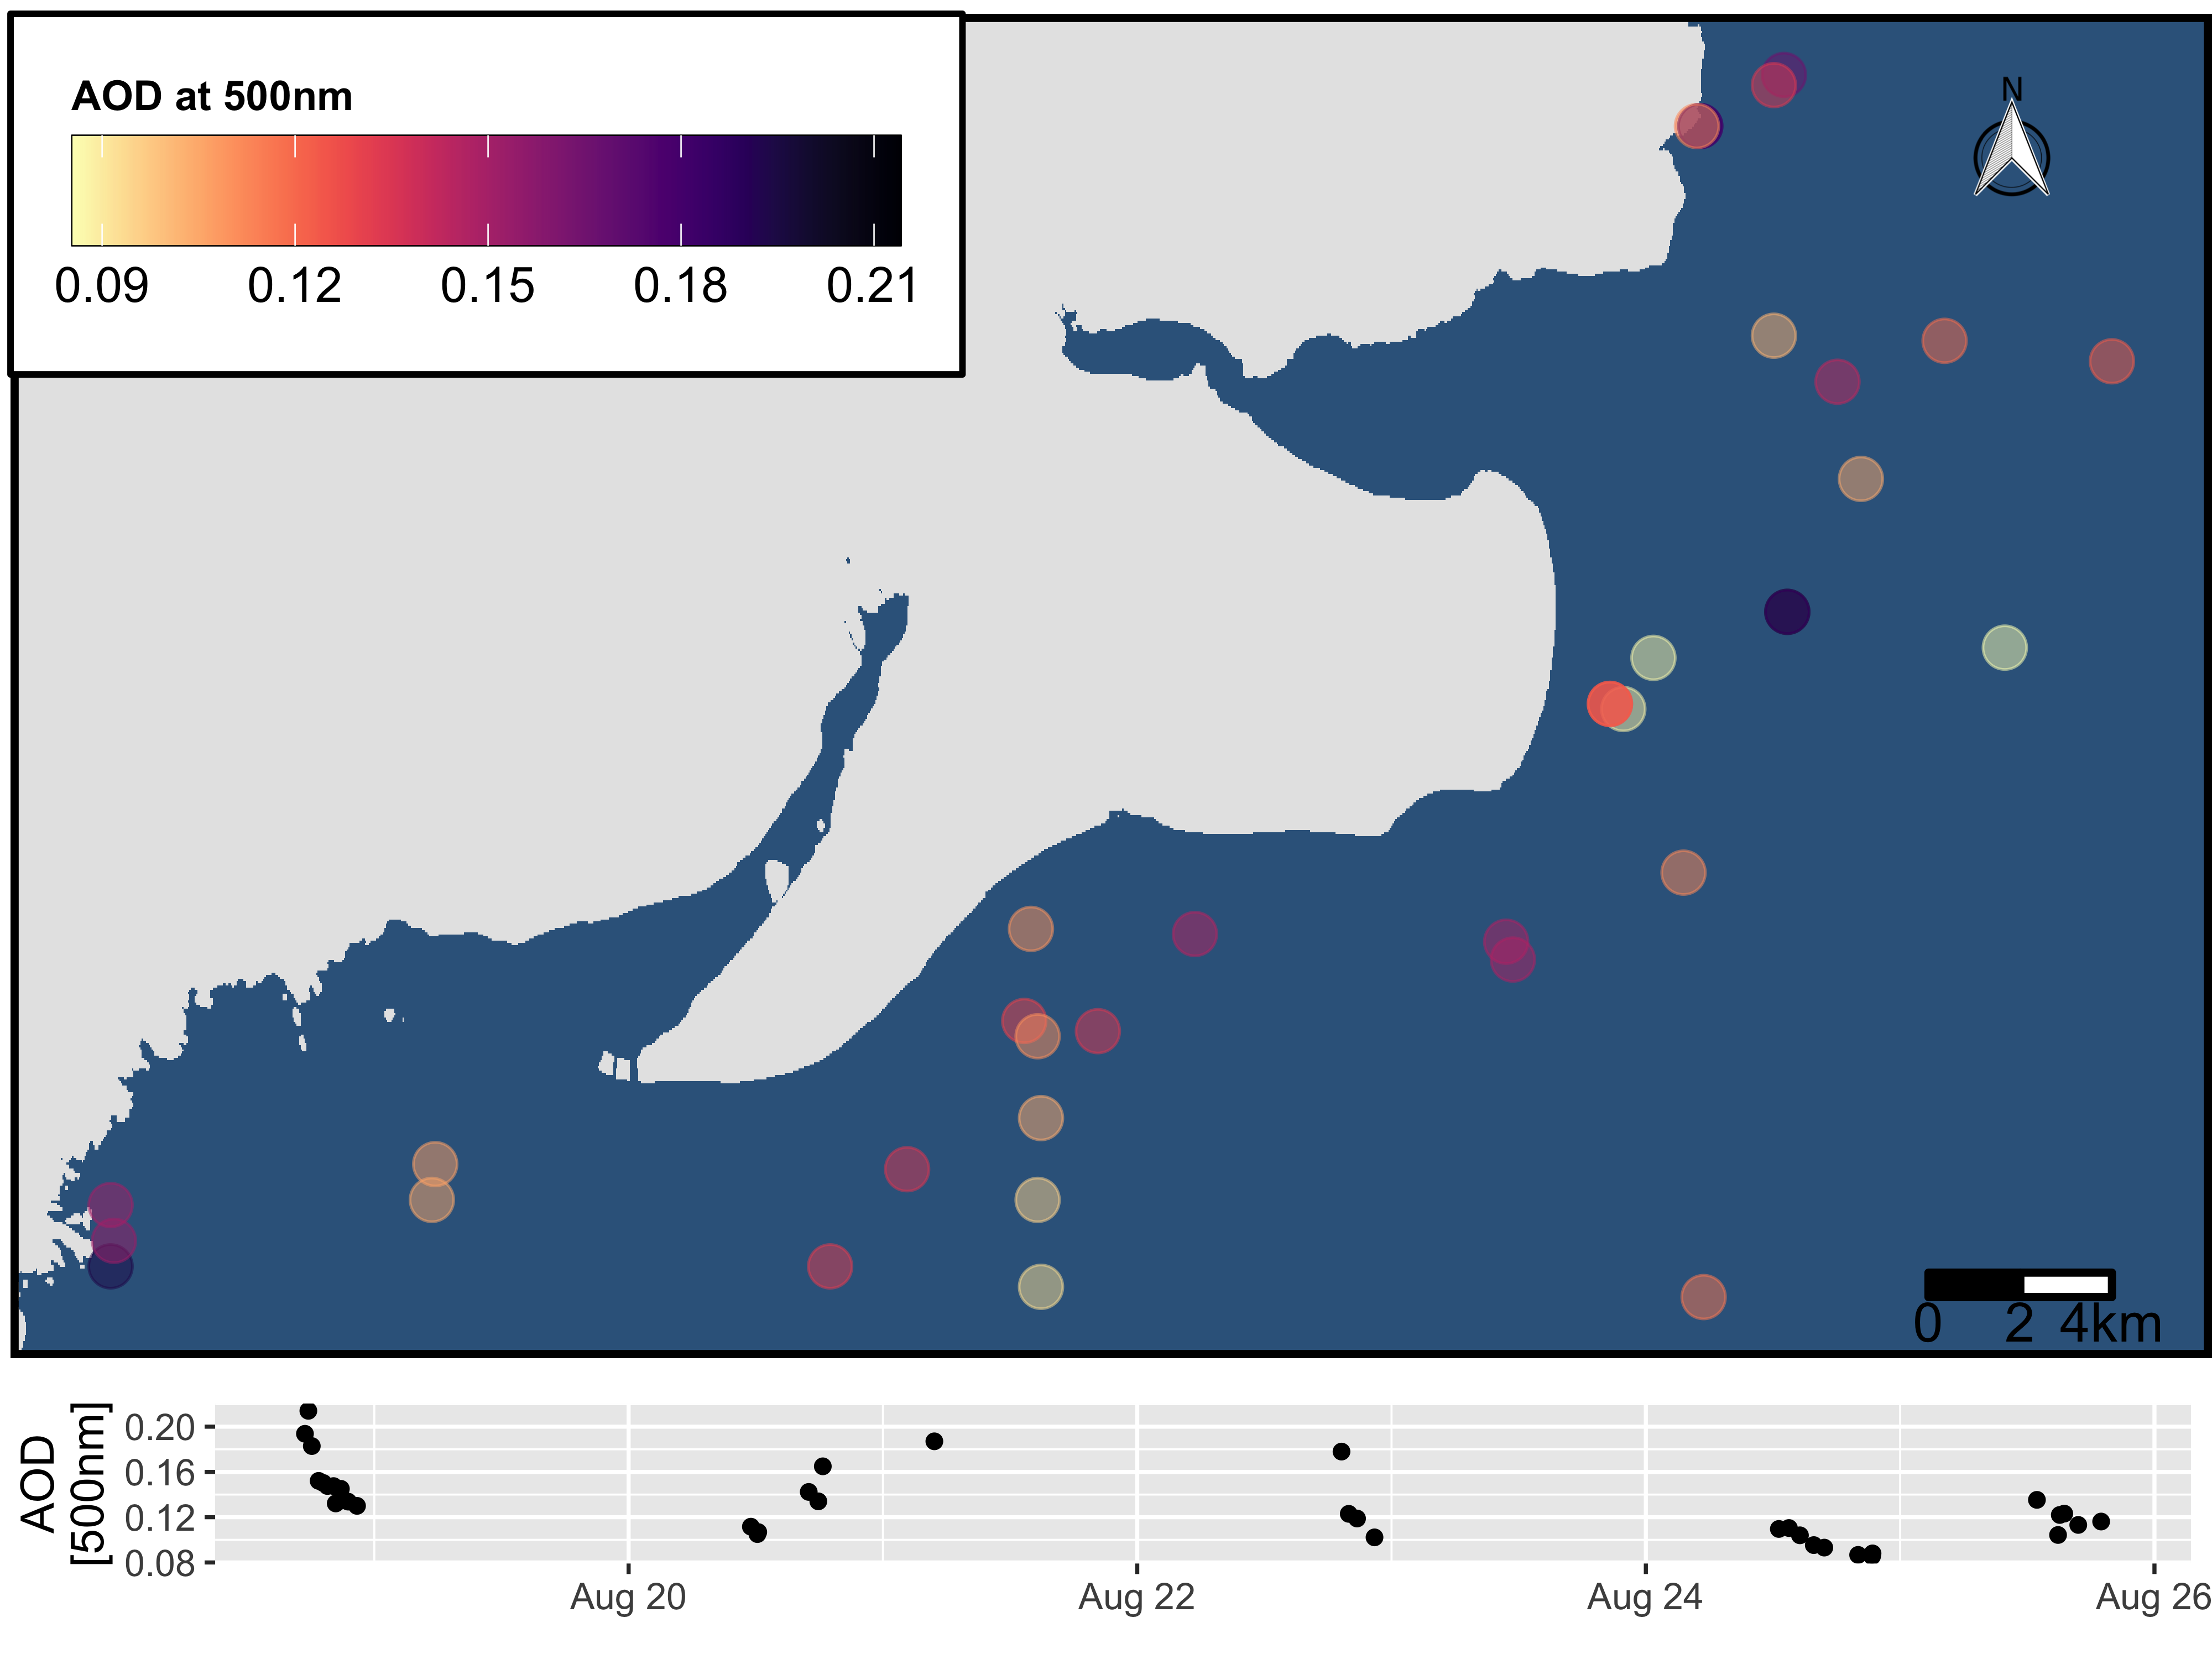
\includegraphics[width=8.3cm]{Figures/fig_AOD.png}
    \caption{Aerosol optical thickness at 500 nm between 17 and 25 August 2020 obtained from Microtops measurements made on two small vessels }
    \label{fig:AOD}
\end{figure}

 
Figure~\ref{fig:AOD} shows no discernible spatial pattern, but a decrease in AOD [500 nm] with time (WHY ? DO WE HAVE THE WIND DIRECTION ?). The median was computed for all the remaining sequences. A summary of these values is presented in Table \ref{table:AOT}. 
 

\begin{table}[t]
\caption{Summary of the atmospheric parameters derived from the two sun photometers.}
\centering
\begin{tabular}{ cccccc  }
\tophline
 & AOD [500nm] & AOD [870nm] & Angstrom exponent [440-870nm] & Water vapor (cm) & n\\
\middlehline
mean & 0.130 & 0.060 & 1.40 & 2.20 & 5.4 \\
std & 0.032 & 0.014 & 0.21 & 0.75 & 1.4 \\
min & 0.087 & 0.042 & 1.00 & 1.10 & 3.0 \\
max & 0.210 & 0.120 & 1.80 & 3.40 & 8.0 \\
\bottomhline
 \end{tabular}
 \label{table:AOT}
\end{table}

 
For perspective, over the deep ocean, Ahmad et al. (2010) mentioned typical AOD values at 870nm to around 0.086. Smirnov et al. (2009) found globally averaged oceanic AOD values of 0.108 at 500nm and 0.597 for the Angstrom exponent. Using all Maritime Aerosol Network data available in 2020 (https://aeronet.gsfc.nasa.gov/new\_web/maritime\_aerosol\_network.html), we split the dataset in coastal and oceanic data using a threshold of 100km from the nearest shore. For the coastal (oceanic) data, we found a mean AOD [500nm] of 0.151 (0.173), a mean AOD [870nm] of 0.090 (0.136) and a mean Angstrom exponent of 1.161 (0.609). In our case, all angstrom exponents were above one, representing a strong dominance of fine aerosols, continental in nature. Spectral shapes were monotonically decreasing towards longer wavelengths with an absence of blue-absorbing aerosols (Mobley et al. 2016).

\subsection{Laboratory analysis of discrete water samples} \label{labo}
All together, the dataset contains 280 water samples. Depending on the project and year of sampling, all, or a subset of the following parameters were measured in the laboratory:

\subsubsection{Salinity}
Salinity (in PSU) was measured using a Guildline Portasal model 8410A salinometer. The average of three readings was taken as the final value.

\subsubsection{Nutrients}
Nutrients were analyzed by Jean-Éric Tremblay's team (Laval University) for CHONe and Wise. Colorimetric determinations of nutrients were performed on an Autoanalyzer with routine methods (see Tremblay et al. 2008).

\subsubsection{Spectrophotometric measurements}
CDOM absorption

CDOM absorbance OD(λ) was measured using the same method as described in Belanger et al. (2017) and \citep{Araujo2022}. Seawater was filtered under low vacuum on 47 mm glass fiber filter (Whatman, GF/F 0.7 mm nominal pore size), which was pre-ashed for 2 h at 450℃ and pre-rinsed with 50 mL of MilliQ water. CDOM absorbance was measured with a Perkin Elmer double-beam Lambda-850 spectrophotometer using a 10 cm quartz cell between 220 and 800 nm against nano pure water. Absorption coefficients were then calculated according to:
\begin{equation}
%     aℊ(λ) = 2.303 OD(λ)/ι
a_g(\lambda) = \frac{2.303 OD(\lambda)}{L}
\label{eq:ag}
\end{equation}
where $a_g(\lambda)$ is the absorption coefficient of CDOM (m$^{-1}$) at wavelength $\lambda$, $OD$ is the absorbance measured at $\lambda$, and $L$ is the pathlength of the optical cell (0.1~m).

Particulate absorption

Measurements of particulate absorption were performed using the filter-pad technique, as described in Bélanger et al. (2017) and and \citep{Araujo2022}. A known volume of the water sample (in two to five replicates) was filtered through Whatman GF/F glass fiber filters shortly after sampling (< 3h). Each filter was then placed in the center of a 150 mm integrating sphere equipped with a spectralon filter holder (see Röttgers and Gehnke 2012 for technical details). The optical depth OD(λ) of the particles retained on the filter was then measured using a Perkin Elmer Lambda-850 spectrophotometer, from 300 to 800 nm at 1 nm resolution. Optical depth was converted to the spectral particulate absorption coefficient, ap(l)(m21), using

ap(λ) = 2.303 OD(λ) A/V OD(λ)-ODblank(λ)/β

where ODblank is the optical density of a blank filter, A is the clearance area of the particles on the filter (m2), V is the volume of sample water filtered (m3), and β is the pathlength amplification factor. The relationship between β and OD derived experimentally by Stramski et al. (2015) was used. After the OD scanning, phytoplankton pigments were extracted for 18–24h using methanol (Kishino et al. 1985), which removed nearly all pigments (95\% of sample). The filter was then placed again in the integrating sphere to measure the absorption coefficient of nonalgal particles, aNAP. The absorption coefficient of phytoplankton aø was obtained by subtracting aNAP from the total particulate absorption coefficient.

\subsubsection{ Chlorophyll-a and phaeopigments: in vitro fluorometric determination}
Triplicate subsamples for Chl-a and phaeopigments concentration determination were filtered following the filtration protocol described by Trees et al. (2002). Chl-a concentrations were measured using a Turner Design 10-AU fluorometer, following a 24-h extraction in 90\% acetone at 4ºC in the dark without grinding (acidification method: Parsons et al. 1984). The final value from triplicates was determined considering their average, within a confidence interval of 95\%. Pigment concentrations were derived as recommended by Jefrrey and Humphrey (1975).

\subsubsection{Pigments: High Performance Liquid Chromatography (HPLC)}
Measurements of pigments were performed using High Performance Liquid Chromatography (HPLC) at ISMER, according to Zapata et al (2000). Water samples were filtered through 25 mm Whatman GF/F glass fiber filters (0.7 mm nominal pore size) and stored in cryogenic vials at -80℃. The internal standards (IS) of apo-caroten were stored at -20℃. The whole extraction procedure was conducted in the dark under a green light to avoid the degradation of the photosynthetic pigments. Samples were kept cool during the whole extraction procedure in an ice-filed container. Filters were placed in 15 ml tubes containing 3 ml of 95\% methanol. After letting the SI at room temperature for 5 minutes, a 50 µL volume was injected in the 15 ml tube containing the sample as well as in the blank sample. The samples were then crushed using a sonicator QSonica Q125 3 to 4 times at 5 seconds.  Once sonicated, the samples were centrifuged in a Eppendorf cooling centrifuge 5430R at 6500 RPM for 5 minutes at 4℃. Samples were filtered through a PTFE 0.2 mm encapsulated filter. The 13 mm capsule was screwed on a glass syringe and washed with acetone and methanol between each sample. The filtering step ensured to eliminate any impurities and kept only the relevant pigments to be analysed with HPLC. Finally, a small amount of argon was added to the vials in order to limit pigment oxidation caused by oxygen in the air.
 
Samples were placed in the HPLC analyser (Agilent Technologies 1 200 series) according to the method in Galindo et al. (2017) and the results were read with EzChrome Elite Software. A chromatogram representing the absorption peak of pigments in absorbance units (mAU) in relation to retention time (minutes) was generated for each sample. Detection and quantification limits were estimated as described in Bidigare et al. (2011). Peaks having an area under 2000 mAU were eliminated because of identification difficulties. Some pigments where standards were absent from our database were considered as “unknown” and discarded from future analyses. Those “unknows” were too scarce among the samples to allow proper identification. Reading of all pigments was done at 450 nm, except for phaeopigments, which were read at 412 nm because they are undetectable at 450 nm. A small variability was observed in retention time among the samples depending on the vial analyzed.
 
Pigment concentrations were calculated as follow:


CPig = (APig*Vex*Aapo\_blanc) / (C*Vinj*Vfil*Aapo\_ech)
 
where CPig is the individual pigment concentration (µg L–1), APig is the individual pigment peak area, Vex is the extraction total volume (mL), Aapo\_blanc is the apo-caroten peak area in the blank sample, C is the calibration coefficient associated with the pigment (area.µg–1), Vinj is the injected volume (mL), Vfil is the filtered volume (mL) and Aapo\_ech is the apo-carotene peak area in the sample.


\subsubsection{Bacterial and phytoplankton cells count: flow cytometry analysis}
Heterotrophic prokaryotes (Archaea and Bacteria) and <20 µm autotrophs abundances were measured by flow cytometry. For each analysis, duplicate 4 mL subsamples were fixed with glutaraldehyde Grade I (Sigma; 0.1\% final concentration) in the dark at room temperature for 15 min, flash-frozen in liquid nitrogen and then stored at -80°C until analysis. 
 
Samples for heterotrophic prokaryotes enumeration were stained with SYBR Green I (Invitrogen) following Belzile et al. (2008). Bacteria (and Archaea) were counted with a CytoFLEX flow cytometer (Beckman Coulter) using the blue laser (488 nm). The green fluorescence of nucleic acid-bound SYBR Green I was measured at 525 nm (525/40 nm BP). The cytograms obtained were analyzed using CytExpert v2.3 software and the same regions of the side scatter vs. green fluorescence plots were ascribed to low nucleic acid (LNA) and high nucleic acid (HNA) bacteria for the whole dataset.
 
Samples for <20 µm autotroph abundances (i.e. phycoerythrin-containing cyanobacteria, phycocyanin-containing cyanobacteria and autotrophic eukaryotes) were analyzed using a CytoFLEX flow cytometer (Beckman Coulter) fitted with a blue (488 nm) and a red laser (638 nm). Using the blue laser, forward scatter, side scatter, orange fluorescence from phycoerythrin (582/42 nm BP) and red fluorescence from chlorophyll (690/50 nm BP) were measured. The red laser was used to excite the red fluorescence of phycocyanin (660/20 nm BP). Polystyrene microspheres of 2 µm diameter (Fluoresbrite YG, Polysciences) were added to each sample as an internal standard. Pico- (<2 µm) and nano-autotrophs (2-20 µm) were discriminated based on a forward scatter calibration using algal cultures. Nano-sized autotrophs containing phycoerythrin or phycocyanin were ascribed to nanocyanobacteria but could have also been cryptophytes or rhodophytes (Kirk 1994).

\subsubsection{Suspended Particulate Matter (SPM)}
SPM were measured according to Bélanger et al. (2017) and \citet{Mabit2022}. Known volumes (V) in liters of seawater (1 L, depending on turbidity) were filtered in triplicate through pre-ashed (1h at 450℃) and pre-weighed (mass M0,mg) 25 mm glass fiber filters (Whatman, GF/F 0.7 mm nominal pore size) at low vacuum (VanDer Linde 1998). Each filter was then rinsed with Milli-Qwater, dried for 24h at 60℃ prior to weighing under a dry atmosphere (mass M1, mg) to obtain the SPM concentration (mgL-1) as:

SPM =(M1 - M0) / V

The fraction of the inorganic matter (PIM) and organic matter (POM) in the total SPM pool was determined using the  lost on ignition (LOI) technique, where the filters were baked for 3h at 500℃ before weighing again.
The average coefficient of variation (CV) for triplicates considering the entire dataset is 17.95\% and 22.45\% respectively for SPM and PIM. CV for individual project are presented in Table  \ref{table:SPMCV}.

\begin{table}[t]
\caption{Coefficient of variation for SPM and PIM.}
\centering
\begin{tabular}{ c|cc  }
\tophline
 & SPM & PIM\\
\middlehline
PMZA-RIKI & 20.21 & 23.71 \\
BSI & 15.70 & 18.79 \\
WISE-Man & 21.87 & 28.48 \\
\bottomhline
 \end{tabular}
 \label{table:SPMCV}
\end{table}

\subsubsection{Total and Dissolved Organic Carbon (TOC, DOC) and Nitrogen (TDN)}
DOC concentration was measured using a Shimadzu TOC-Vcpn carbon analyzer equipped with a TNM-1 module (Total Nitrogen Measurement unit) simultaneously measuring the dissolved nitrogen concentration (DN, inorganic plus organic). Potassium hydrogen phthalate and potassium nitrate were used to standardize DOC and DN measurements, respectively. In addition, samples were systematically checked every seventh sample analysis against Nanopure water (Barnstead Nanopure Infinity) and deep seawater reference from Florida Strait (43-45 µmol C L-1 and 32-33 µmol N L-1) produced by the Hansell’s consensus reference materials (CRM) program. The coefficient of variation on three replicate injections was typically <2\% for DOC and <5\% for DN.

\subsubsection{Phytoplankton taxonomy}
To determine the phytoplankton community composition and abundance, 200 ml of seawater were collected in an amber glass boston bottle at each sampling station. A volume of 0.8 ml of acidified Lugol solution were added in each bottle to fix and preserve the samples until cell counts were done in the laboratory by photonic microscopy (inverted microscope Zeiss Axiovert 10, magnification 400X).Cell identification was made to the lower rank possible (groups, genus and species) and a minimum of 400 cells was enumerated to be statistically significant. Enumeration and calculus were based on Utermöhl and Lund methods. Taxonomy was done for the CHONe (N=20) and WISE-Man project (N=17).

\subsection{Benthic habitats} \label{benthos}
The characterizarion of benthic habitats was done during the WISE-Man project only. The method for the intertidal and infra-lottoral zones is detailed below.
\subsubsection{Intertidal}
A total of 195 stations were samppled at low tide, which covered the principal vegetation communities of the Manicouagan Peninsula: seagrass (Zostera Marina), macroalgae, saltmarsh cordgrass (Spartina alterniflora) and Mediterranenea saltbush (Atriplex halimus). Depending on the station, a combination of biological parameters, sediment core, and bottom reflectance were collected (Figure~\ref{fig:intertidal}).

Vegetation parameters were sampled with 30 cm x 30 cm quadrats. The vegetation percent cover was estimated in the field for each quadrat. The entire vegetation was removed from the quadrat to determine the plant density per m2, the number of photosynthetic active leafs, leaf length, foliar area and the Leaf Area Index (LAI). Data related to leaf (number, length, and foliar area) were obtained from 3 plants (or stem) randomly chosen in each quadrat. Those selected plants were representative of the whole quadrat. Foliar area was determined with ImageJ software. For biomass, the vegetation was rinsed, drained and weighted for wet weight. Vegetation was then placed at 60 degrees C for 48h to 72h until completely dry, and weighted again for dry weight.

Sediment core samples were collected within the first 15 cm of the sediment with a 60 mL truncate syringe. Two replica (A and B) were sampled per site. The core samples were transferred in a sealed cylinder and stored in a cooler until the crew returned. The first 1-2 cm were used for this analysis. Chlorophyll a and phaeopigments concentration in the sediment were measured in the lab with a Fluorimeter TD 10-AU (Christian Nozais lab at ISMER/UQAR). Three readings were made for each replica, which were averaged to give one value per replica.
The granulometry was realized with a laser granulometer, the Mastersizer 3000 (ISMER/UQAR). Three consecutive measurements were made for each sample, and averaged. Detailed method is described in Belzile and Montero-Serrano 2022.

The bottom reflectance was measured ten times over the vegetation-growing season from July 28th  to August 7th.  The plot area was defined to cover a homogeneous part of each vegetation community. Measurements were made with a VIS-NIR spectroradiometer from Analytical Spectral Device Inc (Handheld2-pro model), commonly referred to as the ASD. The instrument had a spectral resolution of ~3 nm covering a spectral range from 325 to 1075 nm and was fitted with a bare fiber optic with a 25° field of view (FOV). The fiber was installed at the end of a rod fixed to a tripod pointing the surface at the nadir at the right height to cover a 0.25 m2 surface. Before each reflectance measurement, a calibrated reference (spectralon plate) with known reflectance value was measured. At least 10 to 15 field spectrometer measurements were taken at random over the vegetation type on each homogeneous plot. This ensured that the random spectral measurements on each plot covered the range of variance present. Remote sensing reflectance was computed following the same method detailed in section 3.1.2 Above-water radiometry.

\subsubsection{Infra-littoral}
To complete the method section we need to decide what diving data we present. To date (jan 2023), we have SVC data in L1, but no complete log information so we don't know where they were taken and the associated surface description.

\section{Data Quality Control and Data Processing}
Add this section here? Example of text taken from Massicote MALINA data paper: "Different quality control procedures were adopted to ensure the integrity of the data. First, the raw data were visually screened to eliminate errors originating from the measurement devices, including sensors (systematic or random) and errors inherent from measurement procedures and methods. Statistical summaries such as average, standard deviation and range were computed to detect and remove anomalous values in the data. Then, data were checked for duplicates and remaining outliers. The complete list of variables is presented in Table xx."

\section{Results}
Examples of plots to show the results. Note that there seem to have outliers here and there...


\begin{figure}[t]
    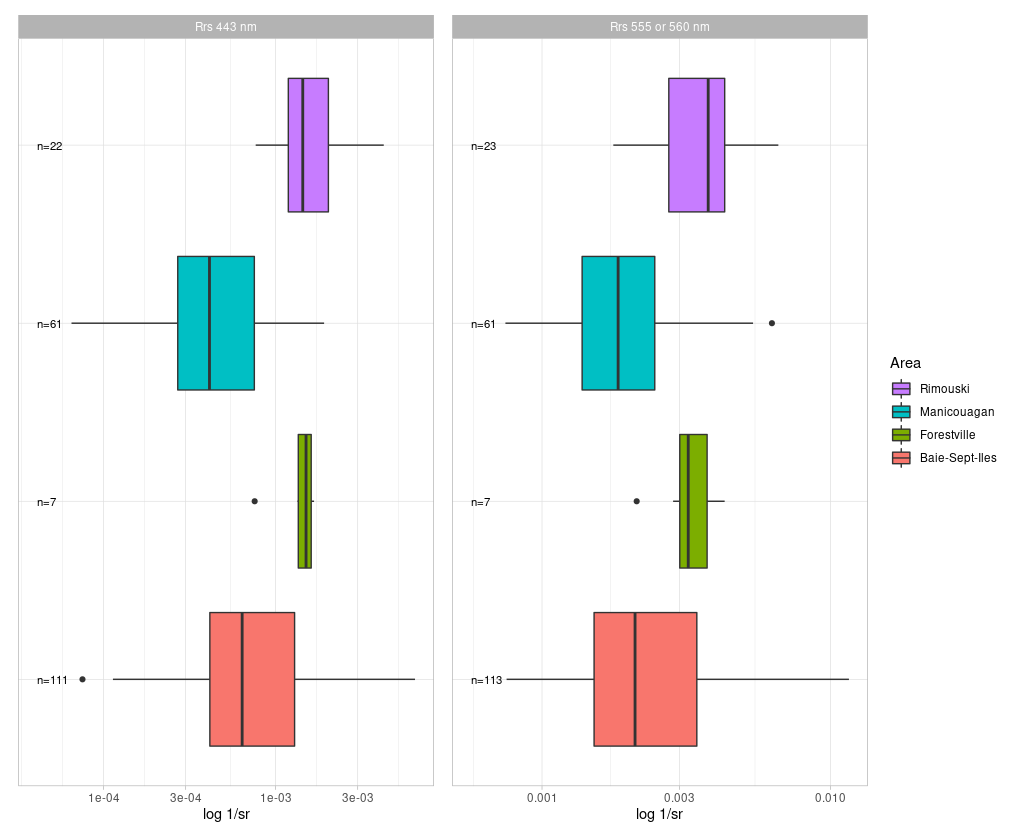
\includegraphics[width=12cm]{Figures/boxplot_Rrs.png}
    \caption{The distribution of remote sensing reflectance at sea surface (Rrs) at 443 nm, and 550/560 nm }
    \label{fig:Rrs443}
\end{figure}

\begin{figure}[t]
    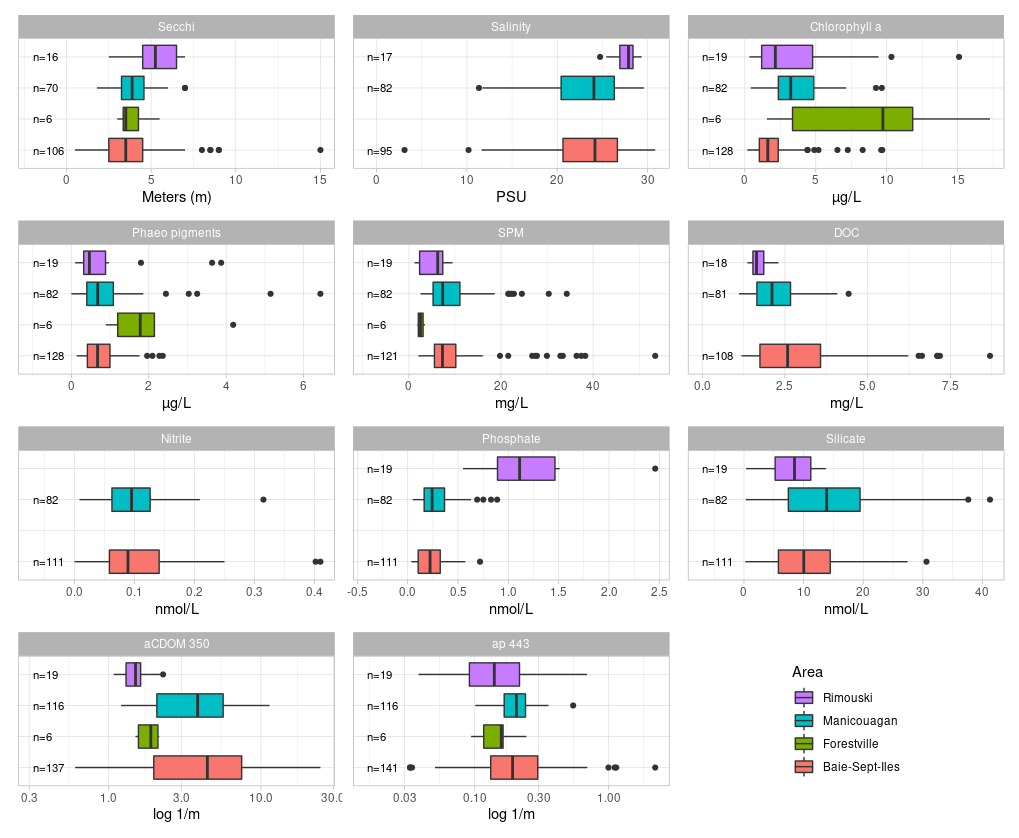
\includegraphics[width=18cm]{Figures/boxplot_biogeochem.png}
    \caption{Variability of biogeochemical and optical parameters measured from water samples}
    \label{fig:biogeochem}
\end{figure}

\begin{figure}[t]
    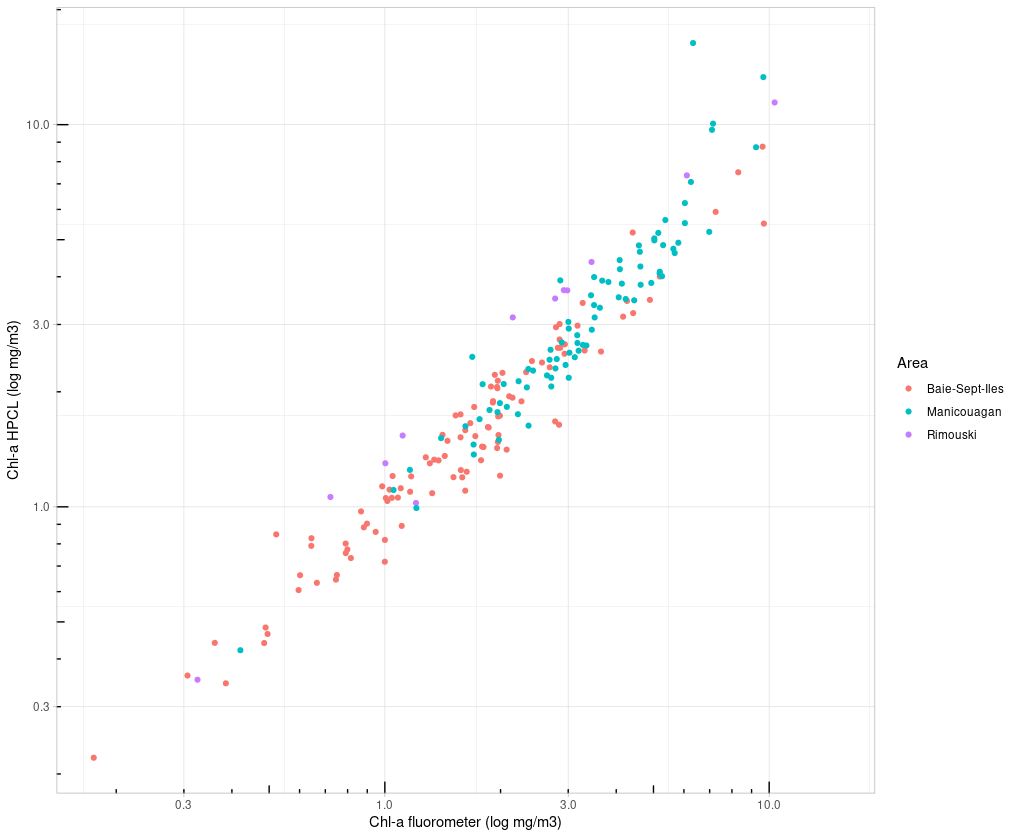
\includegraphics[width=12cm]{Figures/scatter_chla.png}
    \caption{Relationship between chlorophyll a concentration derived with different methods (HPLC and fluorometer), log-transformed to account for their log-normal distribution. }
    \label{fig:chlareg}
\end{figure}

\begin{figure}[t]
    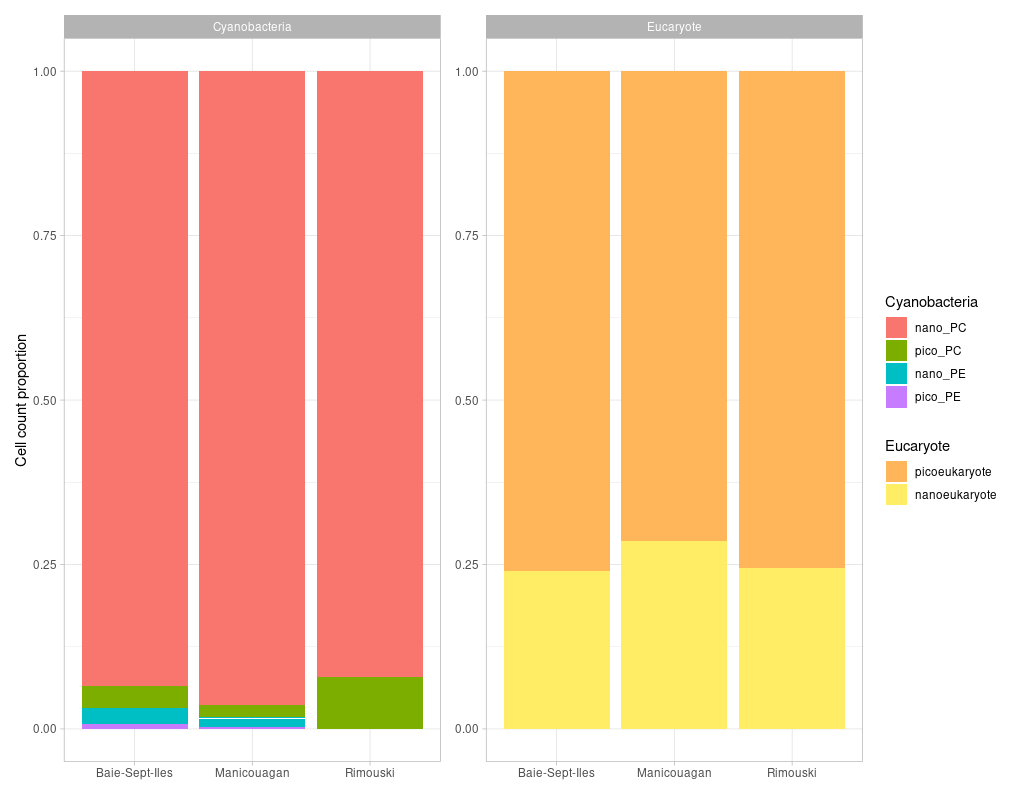
\includegraphics[width=12cm]{Figures/barplot_flowcyto.png}
    \caption{Cell counts of cyanobacteria and euracaryote measured by flow cytometry. nano = nanocyanobacteria, pico =  picocyanobacteria, PC = phycocyanin-rich, PE = phycoerythrin-rich.}
    \label{fig:flowcyto}
\end{figure}

\begin{figure}[t]
    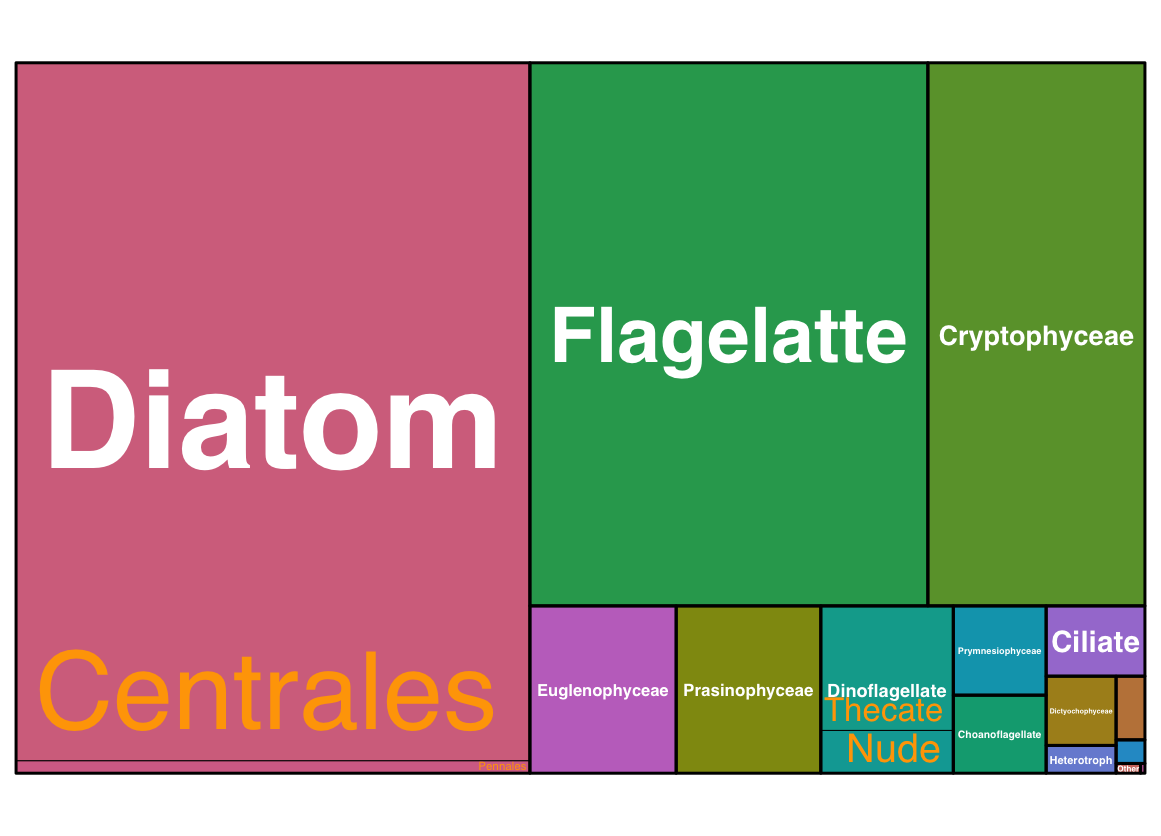
\includegraphics[width=12cm]{Figures/treemap_taxo.png}
    \caption{Taxonomic composition of phytoplankton in the Manicouagan area.}
    \label{fig:treemap}
\end{figure}

\begin{figure}[t]
    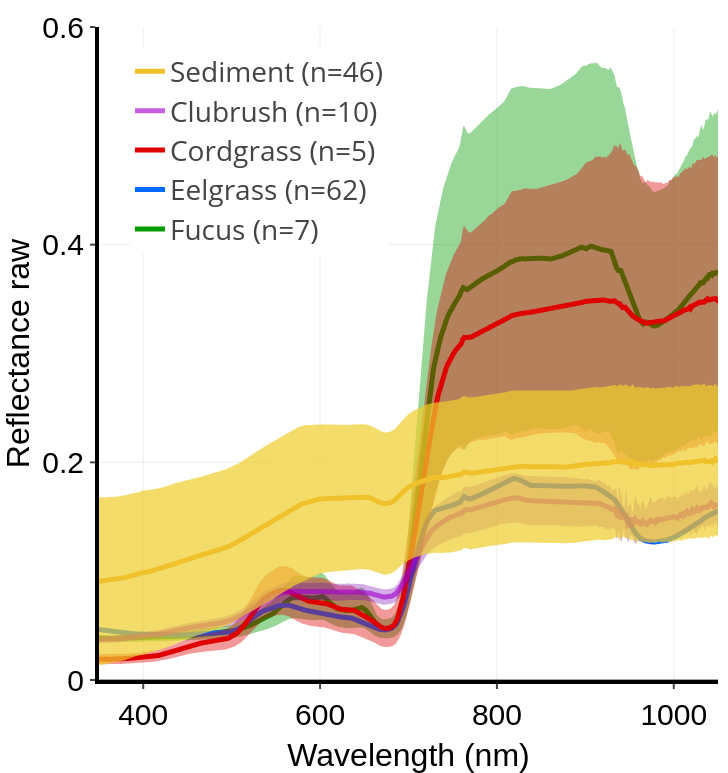
\includegraphics[width=12cm]{Figures/ASD_intertidal.png}
    \caption{Mean reflectance spectra (raw data) of four vegetation species and sediments and their standard deviations (shaded area). n represents the number of station. For the vegetated stations, only stations with more than 50\% species cover were used for the graph. Clubrush = \textit{Bolboschoenus maritimus}, Cordgrass = \textit{Spartina alterniflora}, Eelgrass = \textit{Zostera marina }.}
    \label{fig:asdintertidal}
\end{figure}


\conclusions  %% \conclusions[modified heading if necessary]
TEXT

%% The following commands are for the statements about the availability of data sets and/or software code corresponding to the manuscript.
%% It is strongly recommended to make use of these sections in case data sets and/or software code have been part of your research the article is based on.

\codeavailability{TEXT} %% use this section when having only software code available


\dataavailability %% use this section when having only data sets available
{Most of the data presented in this paper is hosted on SLGO under a collection of csv files. Table xx indicates if the measured parameters is available on the data repository. Table xx indicates the architecture of the data repository, where the data is separated by project and component (optics, biogeochemistry, intertidal). For each project/component, a metadata file is provided in pdf. "Station" files are provided when necessary to retrieve basic information on each station (date, time, latitude, longitude, etc) and can be used as lookup tables to joining of the different csv files together, based on station id. } 


\codedataavailability{TEXT} %% use this section when having data sets and software code available


\sampleavailability{TEXT} %% use this section when having geoscientific samples available


\videosupplement{TEXT} %% use this section when having video supplements available


\appendix
\section{Notation}    %% Appendix A
See Table in GDive and insert here once finished
https://docs.google.com/spreadsheets/d/1CQfSQyPWn0mrdXx9MKMdQom\_vfKphfoMwtqzOkksKIc/edit?usp=sharing

%% \subsection{}     %% Appendix A1, A2, etc.


\section{Additional Figures}\label{appendixfig}  
\begin{figure}
    \centering
    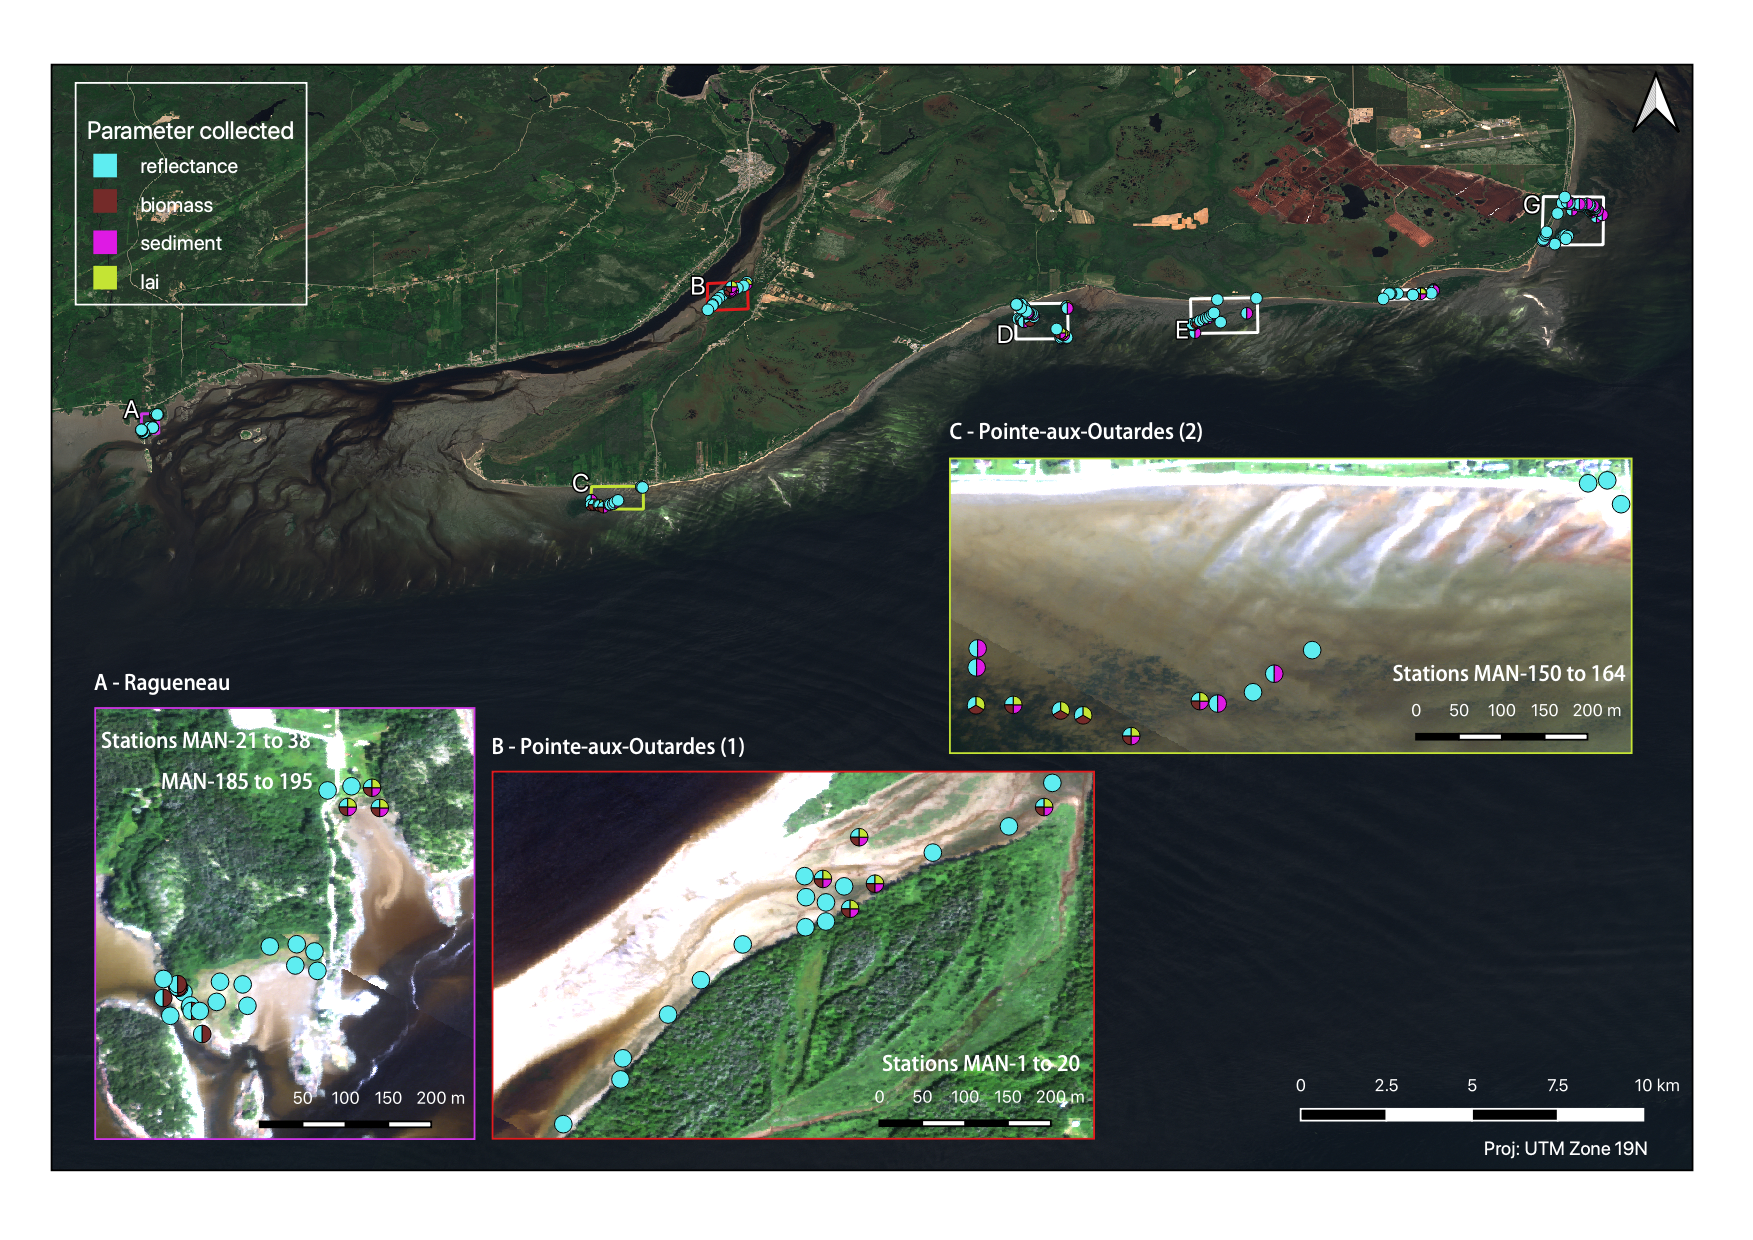
\includegraphics[width=18cm]{Figures/Fig2a_annexe_intertidal__A_B_C_v2.png}
    \caption{Map of stations in the inter-tidal zone visited at low tide between July 27 and August 8, 2019 in the Manicouagan peninsula, showing the different parameters sampled. Insets are zoomed in for three sectors (A, B and C) out of seven. }
    \label{fig:intertidal1_annexe}
    
\end{figure}

\begin{figure}
    \centering
    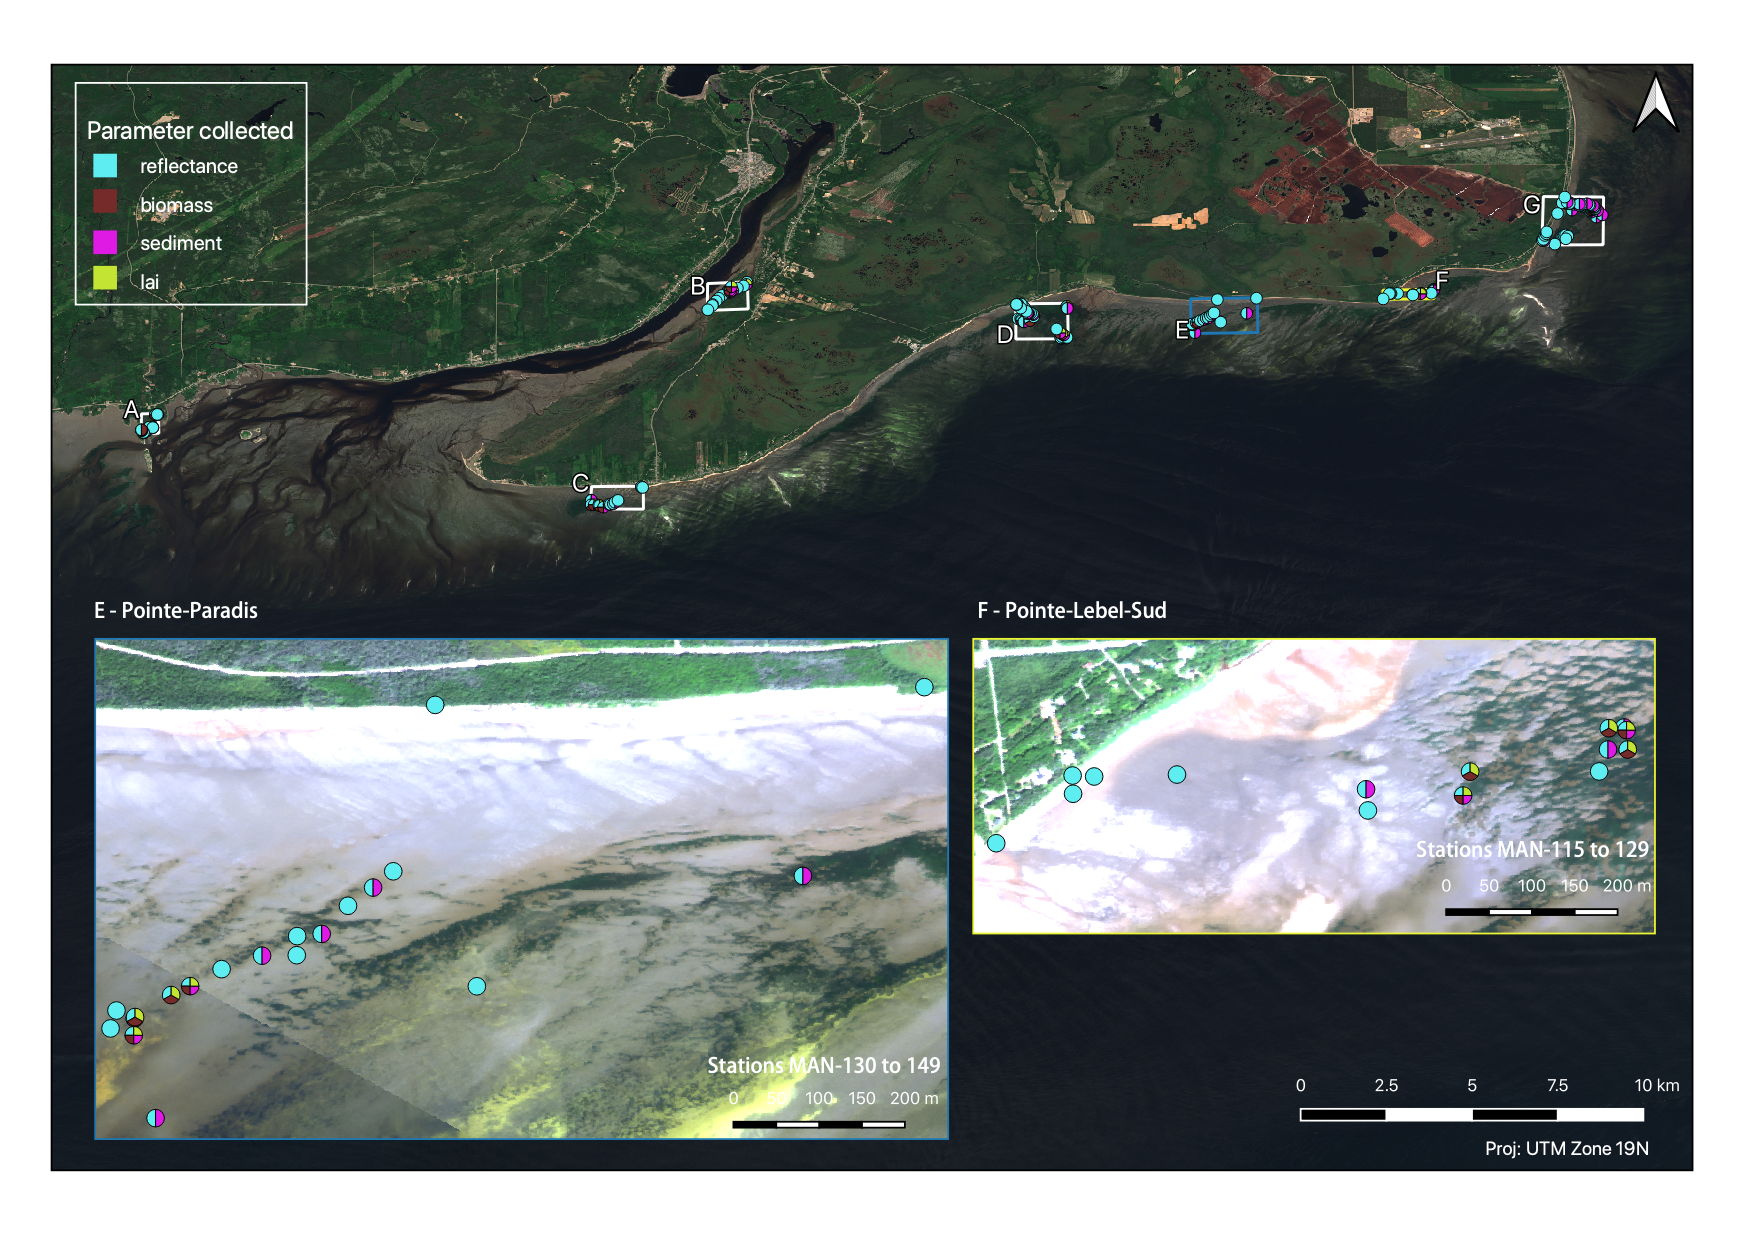
\includegraphics[width=18cm]{Figures/Fig2b_annexe_intertidal_E_F_v2.png}
    \caption{Map of stations in the inter-tidal zone visited at low tide between July 27 and August 8, 2019 in the Manicouagan peninsula, showing the different parameters sampled. Insets are zoomed in for two sectors (E and C) out of seven. }
    \label{fig:intertidal2_annexe}
\end{figure}

%% \subsection{}     %% Appendix A1, A2, etc.


\noappendix       %% use this to mark the end of the appendix section. Otherwise the figures might be numbered incorrectly (e.g. 10 instead of 1).

%% Regarding figures and tables in appendices, the following two options are possible depending on your general handling of figures and tables in the manuscript environment:

%% Option 1: If you sorted all figures and tables into the sections of the text, please also sort the appendix figures and appendix tables into the respective appendix sections.
%% They will be correctly named automatically.

%% Option 2: If you put all figures after the reference list, please insert appendix tables and figures after the normal tables and figures.
%% To rename them correctly to A1, A2, etc., please add the following commands in front of them:

\appendixfigures  %% needs to be added in front of appendix figures

\appendixtables   %% needs to be added in front of appendix tables

%% Please add \clearpage between each table and/or figure. Further guidelines on figures and tables can be found below.



\authorcontribution{TEXT} %% this section is mandatory

\competinginterests{TEXT} %% this section is mandatory even if you declare that no competing interests are present

\disclaimer{TEXT} %% optional section

\begin{acknowledgements}
TEXT
\end{acknowledgements}




%% REFERENCES

%% Since the Copernicus LaTeX package includes the BibTeX style file copernicus.bst,
%% authors experienced with BibTeX only have to include the following two lines:
%%
\bibliographystyle{copernicus}
\bibliography{references.bib}
%%
%% URLs and DOIs can be entered in your BibTeX file as:
%%
%% URL = {http://www.xyz.org/~jones/idx_g.htm}
%% DOI = {10.5194/xyz}


%% LITERATURE CITATIONS
%%
%% command                        & example result
%% \citet{jones90}|               & Jones et al. (1990)
%% \citep{jones90}|               & (Jones et al., 1990)
%% \citep{jones90,jones93}|       & (Jones et al., 1990, 1993)
%% \citep[p.~32]{jones90}|        & (Jones et al., 1990, p.~32)
%% \citep[e.g.,][]{jones90}|      & (e.g., Jones et al., 1990)
%% \citep[e.g.,][p.~32]{jones90}| & (e.g., Jones et al., 1990, p.~32)
%% \citeauthor{jones90}|          & Jones et al.
%% \citeyear{jones90}|            & 1990



%% FIGURES

%% When figures and tables are placed at the end of the MS (article in one-column style), please add \clearpage
%% between bibliography and first table and/or figure as well as between each table and/or figure.

% The figure files should be labelled correctly with Arabic numerals (e.g. fig01.jpg, fig02.png).


%% ONE-COLUMN FIGURES

%%f
%\begin{figure}[t]
%\includegraphics[width=8.3cm]{FILE NAME}
%\caption{TEXT}
%\end{figure}
%
%%% TWO-COLUMN FIGURES
%
%%f
%\begin{figure*}[t]
%\includegraphics[width=12cm]{FILE NAME}
%\caption{TEXT}
%\end{figure*}
%
%
%%% TABLES
%%%
%%% The different columns must be seperated with a & command and should
%%% end with \\ to identify the column brake.
%
%%% ONE-COLUMN TABLE
%
%%t
%\begin{table}[t]
%\caption{TEXT}
%\begin{tabular}{column = lcr}
%\tophline
%
%\middlehline
%
%\bottomhline
%\end{tabular}
%\belowtable{} % Table Footnotes
%\end{table}
%
%%% TWO-COLUMN TABLE
%
%%t
%\begin{table*}[t]
%\caption{TEXT}
%\begin{tabular}{column = lcr}
%\tophline
%
%\middlehline
%
%\bottomhline
%\end{tabular}
%\belowtable{} % Table Footnotes
%\end{table*}
%
%%% LANDSCAPE TABLE
%
%%t
%\begin{sidewaystable*}[t]
%\caption{TEXT}
%\begin{tabular}{column = lcr}
%\tophline
%
%\middlehline
%
%\bottomhline
%\end{tabular}
%\belowtable{} % Table Footnotes
%\end{sidewaystable*}
%
%
%%% MATHEMATICAL EXPRESSIONS
%
%%% All papers typeset by Copernicus Publications follow the math typesetting regulations
%%% given by the IUPAC Green Book (IUPAC: Quantities, Units and Symbols in Physical Chemistry,
%%% 2nd Edn., Blackwell Science, available at: http://old.iupac.org/publications/books/gbook/green_book_2ed.pdf, 1993).
%%%
%%% Physical quantities/variables are typeset in italic font (t for time, T for Temperature)
%%% Indices which are not defined are typeset in italic font (x, y, z, a, b, c)
%%% Items/objects which are defined are typeset in roman font (Car A, Car B)
%%% Descriptions/specifications which are defined by itself are typeset in roman font (abs, rel, ref, tot, net, ice)
%%% Abbreviations from 2 letters are typeset in roman font (RH, LAI)
%%% Vectors are identified in bold italic font using \vec{x}
%%% Matrices are identified in bold roman font
%%% Multiplication signs are typeset using the LaTeX commands \times (for vector products, grids, and exponential notations) or \cdot
%%% The character * should not be applied as mutliplication sign
%
%
%%% EQUATIONS
%
%%% Single-row equation
%
%\begin{equation}
%
%\end{equation}
%
%%% Multiline equation
%
%\begin{align}
%& 3 + 5 = 8\\
%& 3 + 5 = 8\\
%& 3 + 5 = 8
%\end{align}
%
%
%%% MATRICES
%
%\begin{matrix}
%x & y & z\\
%x & y & z\\
%x & y & z\\
%\end{matrix}
%
%
%%% ALGORITHM
%
%\begin{algorithm}
%\caption{...}
%\label{a1}
%\begin{algorithmic}
%...
%\end{algorithmic}
%\end{algorithm}
%
%
%%% CHEMICAL FORMULAS AND REACTIONS
%
%%% For formulas embedded in the text, please use \chem{}
%
%%% The reaction environment creates labels including the letter R, i.e. (R1), (R2), etc.
%
%\begin{reaction}
%%% \rightarrow should be used for normal (one-way) chemical reactions
%%% \rightleftharpoons should be used for equilibria
%%% \leftrightarrow should be used for resonance structures
%\end{reaction}
%
%
%%% PHYSICAL UNITS
%%%
%%% Please use \unit{} and apply the exponential notation


\end{document}
